\cotefile{33}
\scanpage{2}

Nous prendrons comme prétexte la théorie des fonctions $L$ pour développer plus avant le formalisme de la cohomologie étale. Trois parties

a) Continuer l'étude \inserted{de la coh. étale} avec des coefficients de torsion, en développant en particulier, dans ce cadre, \deleted{\unsure{plus}} \deleted{\unsure{uniquement}} avant le formalisme de dualité, \deleted{\unsure{donner}} donnant des formules de Künneth et de Lefschetz.

b) Étendre le formalisme à des coefficients \uline{$l$-adiques}.

c) Appliquer les résultats au formalisme des fonctions $L$.

1°) \uline{Site étale} de $X$ ;
\[
X_{\mathrm{ét}}:\quad\begin{array}{l}
\text{catégorie}\\
\text{familles couvrantes}\\
\text{faisceaux}\\
\text{faisceaux abéliens}\\
\text{cohomologie}
\end{array}
\]

2°) \uline{Exemple} $X-\unsure{\operatorname{Spec}}k$,
\[
X_{\mathrm{ét}}\simeq\widetilde X_{\mathrm{ét}}\simeq\operatorname{Ens}(\pi)
\qquad \pi=\operatorname{Gal}(\bar k/k)
\]

3°) $f:X\longrightarrow Y$ définit
\[X_{\mathrm{ét}}\;\unsure{-}\;Y_{\mathrm{ét}}\]
\[
f^*:\left\{\begin{array}{l}
Y_{\mathrm{ét}}\longrightarrow X_{\mathrm{ét}}\\
\widetilde Y_{\mathrm{ét}}\longrightarrow\widetilde X_{\mathrm{ét}}
\end{array}\right.
\]
\margin{commute aux $\unsure{\varinjlim}$ \unsure{quelc} et aux $\unsure{\varprojlim}$ finies}
\[f_*:\widetilde X_{\mathrm{ét}}\longrightarrow\widetilde Y_{\mathrm{ét}}\]
\margin{commute aux $\unsure{\varprojlim}$ quelc.}
\mspage{1}

\scanpage{3}
% Reading orientation: the principal diagrams are upright after a 180-degree rotation.
\[
M\subset L\qquad \times\,\unsure{M'U}
\]
\[
A\;-
\]
\diagram{\begin{tikzcd}[column sep=large,row sep=large]
X \arrow[d,dash] & \\
k \arrow[r,dash] & Y
\end{tikzcd}}

\diagram{\begin{tikzcd}[column sep=large,row sep=large]
X' \arrow[r] \arrow[dr,"\unsure{\ne\varnothing}"'] & X \arrow[d,dash]\\
& k
\end{tikzcd}}

\diagram{\begin{tikzcd}[column sep=large,row sep=large,
execute at end picture={
\draw (-1.65,0.1) to[bend left=22] (1.65,0.1);
\draw (-1.8,-0.35) to[bend right=18] (-1.8,-1.75);
}]
\unsure{Y} \arrow[d,"f"] & \unsure{Y'} \arrow[l,"h"'] \arrow[d,"f'"'] & \unsure{V'}\\
X & X' \arrow[l,"g",very thick] &\\
\unsure{g(U')} & \unsure{\supset U'\ne\varnothing} &
\end{tikzcd}}

\diagram{\begin{tikzcd}[column sep=large,row sep=large]
\unsure{Y} \arrow[r] \arrow[dr,dash] & X \arrow[d,dash]\\
& k
\end{tikzcd}}
\diagram{\begin{tikzcd}[column sep=large,row sep=large,
execute at end picture={
\draw (0,-1.3) ellipse (0.35 and 0.24);
\draw (-0.2,-1.4)--(0.2,-1.2);
\draw (-0.1,-1.45)--(0.25,-1.25);
\draw (0.55,-1.05)--(0.55,-2.25);
\draw[->] (0.55,-1.05)--(0.55,-2.25);
}]
Y' \arrow[r] \arrow[dr,dash,bend right=10] & X' \arrow[d,dash]\\
k \arrow[r,dash] & k'
\end{tikzcd}}

\diagram{\begin{tikzcd}[column sep=large,row sep=large,
execute at end picture={
\draw (-1.7,0.25) to[bend left=20] (1.65,0.25);
\draw (-1.6,-0.2) to[bend right=10] (-1.5,-1.65);
\draw (1.3,0.05) to[bend left=8] (1.45,-1.7);
\draw (1.45,0.05) to[bend left=8] (1.6,-1.7);
}]
k' & |[draw,circle]| \unsure{X} \arrow[d] & \unsure{X_K|XK} \arrow[l,very thick] \arrow[d,dash,very thick]\\
& k & K \arrow[l,dash]
\end{tikzcd}}

\figure{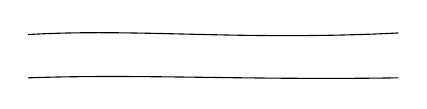
\begin{tikzpicture}
\draw (0,0) .. controls (1.4,0.08) and (2.7,-0.08) .. (4.7,0.02);
\draw (0,-0.55) .. controls (1.4,-0.50) and (2.8,-0.58) .. (4.7,-0.55);
\end{tikzpicture}}
\mspage{2}

\scanpage{4}
\margin{transitivité \ldots\\ $R^i f_*$\\ \uline{Suite spectrale de Leray}}
\margin{\ldots}

4°) Foncteurs fibres

Soit $\xi$ un pt géométrique de $X$
\[
\xi\longrightarrow X,\quad\text{d'où foncteur fibre}
\]
\[
u^*:\widetilde X_{\mathrm{ét}}\longrightarrow\widetilde\xi_{\mathrm{ét}}\simeq(\operatorname{Ens})
\]
La famille des foncteurs fibres est \uline{conservative} : $u:F\unsure{-|\longrightarrow}G$ est un isom ssi les $u_{\bar x}:F_{\bar x}\unsure{-|\longrightarrow}G_{\bar x}$ le sont pour $\forall x\in X$.

d'où les cor. habituels.
\[
F_\xi=\underset{\substack{X'\text{ étale sur}\\X\text{ et pointé}\\\text{par }\xi}}{\unsure{\varinjlim}}F(X')
\]

5°) Localisation stricte
\diagram{\begin{tikzcd}
X' \arrow[d] & \xi \arrow[l] \arrow[dl]\\
X &
\end{tikzcd}}
\[
\underline{\mathcal O}_{X,\xi}\ \deleted{\unsure{\mathcal O_X}}
=\underset{\substack{X'\text{ étale sur}\\X\text{ et }\xi\text{-pointé}}}
{\unsure{\mathop{\mathrm{Lim}}\limits_{\longleftrightarrow}}}
\Gamma(X',\mathcal O_{X'})
\]
\margin{$\left.\begin{array}{l}\text{anneaux stricts}\\\text{locaux ou}\\\text{strict local}\end{array}\right\}\Rightarrow$
i.e. \deleted{\unsure{hensélien et}} hensélien et à corps rés. sép. clos}
\[
\bar X^\xi=\operatorname{Spec}\mathcal O_{X,\xi}
\]
\[
F_\xi=\Gamma(\bar X,F_{\bar X})
\]

6°) Application aux fibres des $R^q f_*(F)$ ; pour $f$ qu. cpt. et qu. sép.

\margin{\uline{NB} 5° et 6° \unsure{n'a} pas vraiment d'analogue \unsure{complet} dans le cas des espaces top. ordinaires \ldots}

\figure{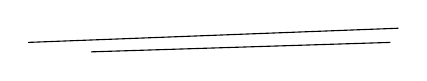
\begin{tikzpicture}
\draw (0,0)--(4.7,0.18);
\draw (0.8,-0.12)--(4.6,0);
\end{tikzpicture}}

7°) \uuline{Théorème fondamental} Soit $f:X\longrightarrow Y$ un morphisme propre, $F$ faisceau \uline{de torsion} sur $X$, alors la formation des $R^i f_*(F)$
\mspage{3}

\scanpage{5}
\margin{. . . .}
\begin{center}- 180 -\end{center}
\hfill n° 391

Alors, (§ 1, n° 3, prop. 8), on aurait $\sum_{k\ne i}q_{ik}^2\geq\frac14+(\frac{\sqrt3}{2})^2=1$, ce qui contredit le lemme 1.

COROLLAIRE 4.-- \uline{Un sommet ne peut appartenir à deux arêtes distinctes d'ordre} $\geq4$.

En effet, (§ 1, n° 3, prop. 8), on a $(\frac{\sqrt2}{2})^2+(\frac{\sqrt2}{2})^2=1$.

Soit $\{i,j\}$ une arête de $X$ ; soit $\underline{M}'=(m'_{hk})$, $(1\leq h\leq\ell,\ 1\leq k\leq\ell,\ h\ne j,\ k\ne j)$, la matrice d'ordre $\ell-1$ définie par $m'_{hk}=m_{hk}$ si $h\ne i$ ou $k\ne i$, $m'_{ik}=m'_{ki}=m_{ik}+m_{jk}$ pour tout $k$ distinct de $i$ et de $j$, $m'_{ii}=m_{ii}=1$. On dit que le schéma de Coxeter $X'$ de $\underline M'$ s'obtient à partir de $X$ \uline{identifiant} $j$ \uline{à} $i$. Les arêtes de $X'$ sont donc les ensembles $\{i,k\}$, $(k\ne j)$, qui sont des arêtes de $X$, les ensembles $\{i,k'\}$, $(k'\ne j)$, tels que $\{j,k'\}$ soit une arête de $X$, et les arêtes $\{k,k'\}$ de $X$ liant des sommets distincts de $i$ et de $j$. Si $k$ est distinct de $i$ et de $j$, on notera que $\{i,k\}$ et $\{j,k\}$ ne peuvent tous deux être des arêtes de $X$, sans quoi elles formeraient avec $\{i,j\}$ un circuit dans $X$ ; on en conclut que si $k$ est \uline{point de ramification} dans $X$, il l'est encore dans $X'$.

LEMME 2.-- \uline{Si l'arête} $\{i,j\}$ \uline{est d'ordre} 3, $G(\underline M')$ \uline{est un groupe fini}.

Notons en effet que si $k$ est distinct de $i$ et de $j$, on ne peut avoir \uline{à la fois} $m_{ik}\geq3$ et $m_{jk}\geq3$, sans quoi les arêtes $\{i,j\}$, $\{j,k\}$, $\{k,i\}$ formeraient un circuit dans $X$. Si on pose $q'_{hk}=-\cos(\pi/m'_{hk})$, $(h,k\text{ distincts de }j)$, on a donc $q'_{ik}=q_{ik}+q_{jk}$ pour $k$ distinct de $i$ et de $j$ ; comme $q_{ii}=q_{jj}=1$ et $q_{ij}=-\frac12$ par hypothèse, on voit que la forme quadratique $B_{\underline M'}$ est telle que pour $x=\sum_{k\ne j}\xi_k e_k$, $B_{\underline M'}(x,x)$ soit égal au nombre obtenu en remplaçant $\xi_j$ par $\xi_i$ dans $q(\xi_1,\ldots,\xi_\ell)$ ; on a donc $B_{\underline M'}(x,x)>0$ par hypothèse si $x\ne0$.
\mspage{4}

\scanpage{6}
\mspage{5}

commute à $\forall$ changement de base $Y'\longrightarrow Y$.

\margin{\uline{NB} Vrai sans hyp. de propreté si $Y'\longrightarrow Y$ est \uline{lisse}, $f$ qu. cpt. qu. sép., et $F$ premier aux car. rés. de $Y$.}

\deleted{8°) \uline{Ex} Morphismes finis $R^q f_* F=0$ si $q\ne0$}

\[
\left\{\begin{array}{ll}
\uline{\text{Ex}} & R^q f_*(F)_{\bar y}\simeq H^q(X_{\bar y},F_{\bar y})\\
\uline{\text{Ex.}} & X\ \underset{\text{sur}}{\text{prop.}}\ k\text{ sép. clos},\quad K'\text{ ext. sép. close de }k,
\end{array}\right.
\]
d'où $X'=X_{K'}$, $F'=F_{X'}$ et $H^i(X,F)\simeq H^i(X',F')$.

\uline{NB} Vrai sans hyp de propreté si $F$ de torsion premier \deleted{\unsure{à la car.}} car $k$.

8°) \uline{Comparaison avec la cohomologie classique}

$X$ préschéma de \unsure{t.f.} sur $\mathbb C$, alors pour $\forall$ $F$ faisceau de torsion sur $X$,
\[
H^q(X,F)\longrightarrow H^q(X^{\mathrm{top}},F^{\mathrm{top}})
\]
est un \uline{isomorphisme}. Résultat analogue pour un morphisme $f:X\longrightarrow Y$, si $f$ est \deleted{\unsure{propre}} \uline{de type fini}.

\margin{Utilise en plus \unsure{résolution sing. pour l'hyp.} de $f$ \deleted{\unsure{de}} de projectivité.}

\margin{\uline{Gaga} plus complet : O.K. pour \deleted{\unsure{Hom}} $\unsure{\operatorname{Ext}^i|\operatorname{Ext}}$ \unsure{de|les} faisceaux de torsion ; équivalence des catégories des faisceaux constructibles algébriques et faisceaux constructibles analytiques qui sont \uline{de torsion}.}

\deleted{\uline{Remarque} Soit $X$ un schéma propre sur une \unsure{algèbre} analytique \inserted{$A=\mathcal O_{Y,y}$} sur $C$, où $Y$ est un espace analytique sur $C$. Alors $X$ ``provient'' d'un espace analytique $X'$ \uline{propre} au dessus d'un voisinage ouvert $Y'$ de $Y$. \deleted{\unsure{À chaque}} $\unsure{\forall}$ faisceau \inserted{de torsion} constr. $F'$ sur $X'$ ``induit'' un \deleted{\unsure{faisceau}} constr. $F$ sur $X$.}

\scanpage{7}
\begin{center}- 179 -\end{center}
\hfill n° 391

conséquences sur les $m_{ij}$ qui permettront de dresser la liste de toutes les possibilités pour les schémas de Coxeter correspondants ; il restera ensuite à voir que ces possibilités sont effectivement réalisées, c'est-à-dire que les groupes correspondants $G(\underline M)$ sont \uline{finis}, (ou encore que la forme $q$ est positive non dégénérée).

LEMME 1.-- \uline{Pour tout} $i$, \uline{on a} $\sum_{j\ne i}q_{ij}^2<1$.

On peut se borner à ne considérer que les indices $j$ pour lesquels $q_{ij}\ne0$, c'est-à-dire ceux qui sont liés à $i$ dans $X$. Si $j$, $j'$ sont deux de ces indices distincts, $\{j,j'\}$ n'est pas une arête, sinon $\{i,j\}$, $\{j,j'\}$ et $\{j',i\}$ formeraient un circuit dans $X$ ; donc $e_j$ et $e_{j'}$ sont \uline{orthogonaux}, et le lemme résulte du fait que, dans $E$, la distance $d$ de $e_i$ au sous-espace vectoriel $F$ engendré par les $e_j$, $(j\text{ lié à }i)$, est donnée par $d^2=1-\sum_j(e_i\mid e_j)^2=1-\sum_{j\ne i}q_{ij}^2$ en vertu du th. de Pythagore, les $e_j$ formant une base orthonormale de $F$.

COROLLAIRE 1.-- \uline{Un sommet de} $X$ \uline{ne peut appartenir qu'à} 3 \uline{arêtes au plus}.

En effet, si $i$ est lié à $h$ autres sommets, les relations $q_{ij}^2\geq1/4$ pour ces sommets $j$ entraînent $h/4<1$ par le lemme 1, donc $h\leq3$.

COROLLAIRE 2.-- \uline{Si} $i$ \uline{appartient à} 3 \uline{arêtes}, \uline{ces arêtes sont d'ordre} 3.

Comme $\cos(\pi/m)\geq\sqrt2/2$ pour $m\geq4$, (§ 1, n° 3, prop. 8), on aurait en effet, dans le cas contraire, $\sum_{j\ne i}q_{ij}^2\geq\frac14+\frac14+\frac12=1$, ce qui contredit le lemme 1.

COROLLAIRE 3.-- \uline{S'il existe une arête d'ordre} $\geq6$, \uline{on a} $\ell=2$.

Soit en effet $\{i,j\}$ cette arête. Si on avait $\ell>2$, un des sommets $i$, $j$, (par exemple $i$), serait lié à un troisième sommet $j'$, puisque $X$ est connexe.
\mspage{6}

\scanpage{8}
\deleted{\unsure{On peut notamment} \unsure{prouver que|trouver que}
$H^i(X,F)\simeq\underset{U\ni y}{\unsure{\varinjlim}}H^i(\deleted{\unsure{X_\xi}}f^{-1}(U),F')$}
\margin{\unsure{Il y a aussi des} \unsure{topos relatifs} du type :}

\uline{Remarque} Soit $f:X\longrightarrow Y$ un ``schéma relatif'' de type fini sur un espace analytique $Y$, d'où $f^{\mathrm{an}}:X^{\mathrm{an}}\longrightarrow Y$. Tout faisceau étale constructible \inserted{de torsion $F$} sur $X^{\deleted{\unsure{\mathrm{an}}}}$ définit un faisceau analytique $F^{\mathrm{an}}$ sur $X^{\mathrm{an}}$, d'où les hom.
\[
\left\{\begin{array}{l}
H^q(X,F)\;\unsure{-}\;H^q(X^{\mathrm{an}},F^{\mathrm{an}})\\
R^q f_*(F)^{\mathrm{an}}\longrightarrow R^q f^{\mathrm{an}}_*(F^{\mathrm{an}})
\end{array}\right.
\]
À prouver que ce sont des \uline{isomorphismes}.

\margin{Devrait aussi se généraliser au contexte rigide analytique \ldots}

\uline{\unsure{Ex.}} Passant à la limite sur les voisinages d'un pt $y\inserted{\in Y}$, on trouverait alors
\[
H^i(X\times_Y\operatorname{Spec}\mathcal O_{Y,y},
 F\otimes\operatorname{Spec}\mathcal O_{Y,y})
\simeq\varinjlim_{U\ni y}H^i((f^{\mathrm{an}})^{-1}(U),F^{\mathrm{an}})
\]
\margin{schéma réellement de t.f. sur $\mathcal O_{Y,y}$}
\margin{$*$}

Par exemple, prenons $X=Y-Z$, $Z$ partie analytique, on en déduit que le calcul des $R^q f_*^{\mathrm{an}}(F^{\mathrm{an}})$ ($F$ faisceau de torsion, mettons loc. cst, sur $Y-Z$) \deleted{\unsure{le calcul}} peut se faire dans le cadre de la \uline{Géom.} \uline{alg.}.
\mspage{7}

\scanpage{9}
% Typed face read after a 180-degree rotation.
\uline{Variétés de groupe}\hfill - 22 -\hfill Tribu n° 62

a) à un hom. d'alg. top. augm. de $\hat P(M)$ dans $\hat P(M)\mathbin{\widehat\otimes}\hat P(M)$

b) à un hom. de coalg. de $U(M)\otimes U(M)$ dans $U(M)$ ; i.e. à une mult. bilin. sur $U(M)$, pour laquelle $\Delta:U(M)\longrightarrow U(M)\otimes U(M)$ soit un hom.

On ne sait si l'on définira en général la notion d'hyperalgèbre.

P. 3-13 : notation $d^{(\unsure{\sigma|\gamma})}_{\alpha,\beta}$ pour éviter la confusion avec les monômes. La formule (30) exprime que le gradué associé de $U(G)$ est $\Gamma(T(G))$.

P. 3-14 : on pense qu'il y a trois niveaux pour les calculs : le niveau intrinsèque (par ex. calculs dans les groupes $G_A$), le niveau semi-intrinsèque (on a un module $M$ et $m$ dans $\hat P(M\times M;M)$), enfin le niveau des coordonnées (on raisonne sur des séries formelles). La formule (31) et les ex. 1 et 2 sont au niveau semi-intrinsèque ; si $m(x,y)\equiv x+y+B(x,y)$ mod. deg. 2, l'alg. de Lie est $M$ avec le crochet $[x,y]=B(x,y)-B(y,x)$ ; en particulier dans $B_m$, on a $m(x,y)=x+y+xy$, d'où $[x,y]=xy-yx$. L'alg. de convolution du gr. additif de $M$ est $(M)$.

La déf. d'un morphisme formel au moyen de coordonnées doit être fait au chap. des variétés formelles.

P. 3-15 à 3-19 : Les groupes $G(A)$ viennent trop tard. En alg. IV, on saura substituer des élts. top. nilpotents tendant vers 0 dans une série formelle, et des élts qconques dans une série restreinte. Regrouper les n° 8 et 9 ; supprimer lignes 1 à 4 haut et 1 à 7 bas. Remplacer $a_k$ par $b_k$ dans (36) et (37).

On pourrait donner les sorites suivants pour les noyaux formels :

a) Bijection $\underline V(A)\simeq\operatorname{Hom}_{\mathrm{alg.top.}}(\hat P_+(\underline V),A)$ pour $A$ alg. top. comm. (pas d'unité exigée) ; la top. sur $\hat P_+(\underline V)$ est la top. faible pour la dualité avec $U(\underline V)$.

b) Tout hom. continu $\sigma:A\longrightarrow B$ donne un $\underline V(\sigma):\underline V(A)\longrightarrow\underline V(B)$.

c) Tout $f:\underline V\longrightarrow\underline W$ donne des $f_A:\underline V(A)\longrightarrow\underline W(A)$.

d) Bijection canonique $(\underline V\times\underline W)(A)=\underline V(A)\times\underline W(A)$.

e) On a $\underline V(A)=\lim_J\underline V(A/J)$ ($J$ idéal ouvert) par constr.

f) Lorsque $A^2=0$, bijection $\underline V(A)\simeq T(\underline V)\mathbin{\widehat\otimes} A$.

Si $G$ est un groupe formel, $G(A)$ est un gr. et $G(\ )$ un hom. de groupes.

g) Si $J$ est un idéal fermé de $A$, on a une suite exacte :
\diagram{\begin{tikzcd}
1 \arrow[r] & G_J \arrow[r] & G_A \arrow[r] & G_{A/J} \arrow[r,dashed] & 1
\end{tikzcd}}
(dernière flèche slt si $\dim G$ finie ou $J$ ouvert). Ajouter prop. 4, (i), (ii).
\mspage{8}

\scanpage{10}
9°) \uline{Th. de spécialisation} Voici \unsure{tjrs} une forme précise : $f:X\longrightarrow Y$ morphisme \uline{propre} et \uline{lisse}, $F$ faisceau de torsion loc. libre sur $X$, premier aux car. résiduelles de $X$, alors les $R^q f_*(F)$ [dont les fibres sont les coh. des fibres \ldots] sont loc. libres.

10°) \uline{Dim.} \uline{cohomologique}.

$X$ de type fini sur $k$ sép. clos, $n=\dim X$, alors
\[
H^i(X,F)=0\quad\text{pour }i\unsure{>|\geq}2n,
\]
($F$ faisceau de torsion sur $X$).

Si $X$ est \uline{affine}, on a $\unsure{=|\simeq}\ H^i(X,F)=0$ pour $i>n$ (th. du type Lefschetz).

La dimension ``topologique'' de $X$ \unsure{passe} donc pour être en général le double de la dimension de Krull --- il y a un abaissement dans le cas affine, qui peut donner des idées fausses.
\mspage{9}

\scanpage{11}
% Typed face read after a 180-degree rotation.
\begin{center}- 137 -\end{center}
\hfill n° 391

injectif, et il résulte alors d'\uline{Alg.} \uline{comm.}, chap. III, § 2, n° 8, cor. 1 du th. 1, que $u$ est lui-même \uline{injectif}, ce qui achève de prouver b).

Le fait que b) entraîne c) résulte aussitôt de ce que $k=S'/\underline m'$ est un $S'$-module de dimension projective $r$, donc $\operatorname{Tor}^{S'}_j(k,M)=0$ pour tout $S'$-module $M$ et pour tout $j>r$.

Enfin, on sait que pour tout idéal premier $\underline p$ de $S$, on a $(\operatorname{Tor}^S_j(M,N))_{\underline p}=\operatorname{Tor}^{S_{\underline p}}_j(M_{\underline p},N_{\underline p})$ quels que soient les $S$-modules $M$, $N$. Appliquant ceci à $M=N=k$ et $\underline p=\underline m$, et notant que $k$ est un $S_{\underline m}$-module, donc aussi $\operatorname{Tor}^S_j(k,k)$, on voit que l'on a $\operatorname{Tor}^S_j(k,k)=\operatorname{Tor}^{S_{\underline m}}_j(k,k)$. Le fait que c) entraîne a) résulte alors de la théorie des anneaux locaux réguliers, (\uline{Alg.} \uline{comm.}, chap. VIII).

COROLLAIRE.-- \uline{Si les conditions de la prop.} 1 \uline{sont vérifiées}, $S$ \uline{est un anneau noethérien régulier de dimension} $r$ ; \uline{pour toute famille d'éléments homogènes} $P_i$ \uline{de} $S$ \uline{vérifiant la condition de la prop.} 1 b), \uline{les degrés} $p_i=\deg(P_i)$ \uline{sont les mêmes à l'ordre près}, \uline{et la série de Poincaré de la} $k$-\uline{algèbre graduée} $S$, (\uline{Alg.}, chap. IV, 3e éd.), \uline{est donnée par} :
\[
(1)\qquad P_S(T)=\prod_{i=1}^r(1-T^{p_i})^{-1}.
\]

La première assertion est vraie pour $S'$, (\uline{Alg.} \uline{comm.}, chap. VIII), donc pour l'algèbre $S$ qui lui est isomorphe. En outre les monômes $P_1^{\nu_1}\ldots P_r^{\nu_r}$ sont linéairement indépendants sur $k$, donc $\dim_k(S_n)$ est égal au nombre de familles d'entiers $(\nu_i)_{1\leq i\leq r}$ telles que $\sum_{i=1}^r\nu_i p_i=n$, ou encore au coefficient de $T^n$ au second membre de (1), ce qui démontre cette formule par définition de la série de Poincaré. Ceci prouve déjà l'invariance des degrés $p_i$ ; on peut aussi le voir directement en notant que les $P_i$ appartiennent nécessairement à $\underline m-\underline m^2$, (sans
\mspage{10}

\scanpage{12}
\margin{cf Artin, Woodshole, pour changement de base}

11) \uline{Supports}
\deleted{\unsure{Désignons|Choisissons} \unsure{donc} \unsure{un|$\forall$} ouvert $U$ de $X$,}

\deleted{\unsure{a}} Faisceau final : $X/X$ lui-même \qquad $X(X')=\{e\}$

Les sous faisceaux du faisceau final sont les ouverts de $X$.

\deleted{Support d'un \unsure{f}}
\deleted{Si $F$ est un \unsure{fai}}

La catégorie des faisceaux $F$ sur $X$ qui sur $U$ sont le faisceau final équivaut à la catégorie des faisceaux sur $Y=X-U$, par le foncteur image directe.

De $=$, faisceaux abéliens sur $X$ nuls sur $U$ $=$ faisceaux abéliens sur $Y$.

Support d'un faisceau abélien

\deleted{$\Gamma_Y(F)\subset\Gamma(F)$ \unsure{Défin.}}

Support d'une section d'un faisceau abélien
\[
\Gamma_Y(F)\subset\Gamma(F)
\]
\[
\underline\Gamma_Y(F)\subset F
\qquad
\underline\Gamma_Y(F)(X')=\Gamma_{Y'}(X',F')
\]

Foncteurs dérivés
\[
\left\{\begin{array}{l}
H^i_Y(X,F)\simeq\operatorname{Ext}^i(X;\mathbb Z_Y,F)\\
\underline H^i_Y(F)\simeq\underline{\operatorname{Ext}}^i(\mathbb Z_Y,F)\\
\phantom{\underline H^i_Y(F)}\text{''}\ R^{i-1}u_*(F|U)\quad\text{si }i\geq2
\end{array}\right.
\]
\margin{si $i=0$ ou $1$, on trouve le noyau et conoyau de $F\longrightarrow u_*(F)$}
\margin{cf SGA 1962 ou Notes Hartshorne 1961}
Suite $\left\{\begin{array}{l}\text{exacte}\\\text{spectrale}\end{array}\right.$ \ldots

12) \uline{Pureté}
$Y\subset X$ réguliers, $\operatorname{codim}_X(Y)=p$ en chaque pt de $Y$
\diagram{\begin{tikzcd}
Y \arrow[dr,dash,"\text{lisse}"'] & & X \arrow[dl,dash,"\text{lisse}"]\\
& k &
\end{tikzcd}}

\margin{\deleted{$\unsure{X}$ \unsure{lisse}}}
\margin{Donner définition de la classe fondamentale locale}
\[
\left\{\begin{array}{lll}
\underline H^i_Y((\mathbb Z/n\mathbb Z)_X)&=0&\text{si }i\ne2p\\
&\simeq\mu_n^{\otimes(-p)}&\text{si }i=2p
\end{array}\right.
\]
\margin{$n$ premier aux car. résiduelles de $Y$}
\mspage{11}

\scanpage{13}
\begin{center}- 194 -\end{center}
\hfill n° 391

5. \uline{Systèmes de type} $A_\ell$, $(\ell\geq1)$.

(I) Considérons dans l'espace $V=R^{\ell+1}$ l'intersection du réseau $L_0$, (n° 4), et de l'hyperplan $V'$ d'équation $\sum_{i=1}^{\ell+1}\xi_i=0$ ; c'est un réseau $L'_0$ dans $V$ ; la valeur minima de $(u\mid u)$ dans $L'_0$ est 2 et elle est atteinte pour les vecteurs de la forme $\varepsilon_i-\varepsilon_j$, $(i\ne j,\ 1\leq i\leq\ell+1,\ 1\leq j\leq\ell+1)$. Montrons que l'ensemble $R$ de ces vecteurs est un \uline{système de racines}, (évidemment réduit), dans $V'$. En effet, il est clair que pour $u,v$ dans $R$, $2(u\mid v)/(u\mid u)$ est entier puisque $(u\mid u)=2$ et la conclusion résulte du n° 4. Le nombre des racines $n$ est $\ell(\ell+1)$.

(II) Posons :
\[
\alpha_1=\varepsilon_1-\varepsilon_2,\quad
\alpha_2=\varepsilon_2-\varepsilon_3,\ldots,\quad
\alpha_\ell=\varepsilon_\ell-\varepsilon_{\ell+1}.
\]
Il est immédiat que tout élément de $R$ est combinaison linéaire des $\alpha_i$, $(1\leq i\leq\ell)$, à coefficients tous $\geq0$ ou tous $\leq0$ ; donc, (§ 6, n° 7, cor. 3 de la prop. 14), les $\unsure{\alpha_i}$ forment un système de \uline{racines simples} $S$ de $R$. En outre, on a $\|\alpha_i\|^2=2$ pour tout $i$, $(\alpha_i\mid\alpha_{i+1})=-1$ pour $1\leq i\leq\ell-1$ et $(\alpha_i\mid\alpha_j)=0$ pour $j>i+1$ ; le schéma de Dynkin de $R$ est donc du type $A_\ell$, ce qui montre que $R$ est irréductible.

(III) En vertu du § 8, n° 3, formule (4), on a $h=n/\ell=\ell+1$.

(IV) L'ordre de la plus grande racine est $h-1=\ell$, (§ 8, n° 5, prop. 6). Or, $\varepsilon_1-\varepsilon_{\ell+1}=\alpha_1+\alpha_2+\ldots+\alpha_\ell$ est une racine positive d'ordre $\ell$ ; donc c'est la plus grande racine $\tilde\alpha$, (§ 6, n° 6, prop. 13). Elle est orthogonale à toutes les racines simples sauf à $\alpha_1$ et $\alpha_\ell$, et on a $(\tilde\alpha\mid\alpha_1)=(\tilde\alpha\mid\alpha_\ell)=1$.
\mspage{12}

\scanpage{14}

\figure{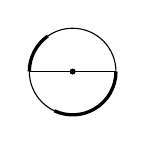
\begin{tikzpicture}[scale=.55]
\draw (0,0) circle (1);
\draw (-1,0)--(1,0);
\fill (0,0) circle (.07);
\draw[line width=1.2pt] (-1,0) arc (180:125:1);
\draw[line width=1.2pt] (1,0) arc (0:-115:1);
\end{tikzpicture}}

NB
\[
\mu_n=\operatorname{Ker}(G_m\xrightarrow{n}G_m)
\]
\[
\mu_n(X')=\deleted{\operatorname{Ker}}\,{}_n\Gamma(X',\mathcal O_{X'})^*
\]
\margin{$\mu_n$ fini plat sur $X$.}

Si $n$ premier aux car de $X$, $\mu_{nX}$ est \uline{étale} sur $X$
loc. isom. (pour top. étale) à $\mathbb Z/n\mathbb Z$. \unsure{Il n'faut|Il ne faut}
surtout pas les confondre. Les $\mu_{nX}^{\otimes d}$
($d\in\mathbb Z$) sont donc définis, et sont \inserted{loc} isomorphes à $(\mathbb Z/n\mathbb Z)_X$
[le choix d'une section primitive de $\mu_n$ définit des isom
$\mu_{nX}^{\otimes d}\simeq(\mathbb Z/n\mathbb Z)_X$, multipliant cette
section par $\lambda\in\mathbb Z/n\mathbb Z$ multiplie l'isom
précédent par $\lambda^d\ldots$].
\uline{Dém} presque immédiate par th. du changement de base\ldots

\margin{\fbox{Pureté ``absolue''}}
\uline{Pb} sans hypothèse de lissité remplacée par hyp.
de régularité. O.K. \inserted{pour \unsure{bons préschémas}}
pour corps car. \unsure{0} quand on
dispose de la résolution des singularités (Artin).

Il y a aussi un th de pureté relatif sur
une base quelconque\ldots

\deleted{13)}

\deleted{13) \uline{Les} $R^i_!f_*(F)$.}
\margin{Extension aux div. à croisements normaux\ldots}
\deleted{Morphismes \unsure{compactifiables} $f:X\longrightarrow Y$.
La factorisation
\diagram{\begin{tikzcd}
X\arrow[r,"i"]&\overline X\arrow[r,dash,"\bar f"]&\unsure{Y}
\end{tikzcd}},
où $i$ \unsure{imm.}}

\mspage{13}

\scanpage{15}

\begin{center}-- 193 --\end{center}
\hfill n$^{\circ}$ 391

(I)\quad Les racines et leur nombre.

(II)\quad Un système de racines simples $S$.

(III)\quad Le nombre de Coxeter.

(IV)\quad La plus grande racine, (relative à $S$), et les racines de $S$ qui ne lui
sont pas orthogonales ; en joignant ces dernières, (dans le schéma de Dynkin),
par un trait pointillé à un point hors du schéma représentant la plus grande
racine, (affecté s'il y a lieu de la longueur de cette dernière), on obtiendra
ce qu'on appelle le \uline{schéma de Dynkin complété}.

(V)\quad Les coracines et la forme bilinéaire canonique, (proportionnelle à la
forme métrique $(x|y)$ de $V$).

(VI)\quad Les poids fondamentaux, (relatifs à $S$).

(VII)\quad La somme des racines positives, (pour $S$).

(VIII)\quad Le groupe $\Gamma(R)/\Gamma_0(R)$ et l'indice de connexion.

(IX)\quad Les exposants, (et éventuellement les invariants symétriques).

(X)\quad L'ordre du groupe de Weyl, (et éventuellement sa structure).

(XI)\quad Les automorphismes du schéma de Dynkin.

Pour chacun des 9 types de schémas de Dynkin, ces données seront rassemblées
dans les planches II à X, en les ordonnant de façon uniforme comme ci-dessus.

\mspage{14}

\scanpage{16}

\deleted{ouverte, et $\bar f$ propre. Ex] morphisme
quasi-projectif sur $Y$ loc. noeth.}

13) \uline{Faisceaux} \uline{constructibles}

Faisceaux loc. \deleted{isom.} constants

Faisceaux constructibles : en général, il est
loc. constant : fibres \deleted{finies} de t.f.
sur des ens loc fermés cons. qui partitionnent
$\unsure{U|X}$. Dans le cas noethérien, critère
par adhérences \unsure{d'un} \unsure{pt} \deleted{\unsure{générique}}.

\uline{Th.}\quad Si $f:X\longrightarrow Y$ \uline{propre}, $Y$ \uline{loc noeth},
alors pour $\unsure{\forall|\text{tt}}$ faisceau \uline{de torsion}
\uline{constructible} $F$ sur $X$, les $R^i f_*(F)$
sur $Y$ sont constr.

\uline{Cor.}\quad $X$ propre sur un corps sép. clos
$k$. Alors pour $\unsure{\forall|\text{tt}}$ $F$ de torsion
constructible sur $X$, les $H^i(X,F)$ sont
des groupes finis.

\uline{Remarque}\quad \unsure{Question} de la généralisation

\mspage{15}

\scanpage{17}

\begin{center}-- 192 --\end{center}
\hfill n$^{\circ}$ 391

2) Le réseau $L_1$ est le sous-$Z$-module de $L_0$ formé des $x=\sum_{i=1}^n\xi_i\varepsilon_i$ tels que
$\sum_{i=1}^n\xi_i$ soit \uline{pair} ; comme $\xi_i$ et $\xi_i^2$ ont même parité, il revient au même de dire
que $(x|x)$ est \uline{pair}. Il est engendré par les $\varepsilon_i\pm\varepsilon_j$, $(i\ne j)$.

3) Le réseau $L_2=L_0+Z.(\frac12\sum_{i=1}^n\varepsilon_i)$ ; il revient au même de dire que les vecteurs
$x=\sum_{i=1}^n\xi_i\varepsilon_i$ de $L_2$ sont ceux qui vérifient les relations :
\[
(4)\qquad 2\xi_i\in Z,\quad \xi_i-\xi_j\in Z\quad\text{quels que soient }i,j.
\]
Comme $(\varepsilon_k|\frac12\sum_i\varepsilon_i)=\frac12$ pour tout $k$, et
$\|\frac12\sum_i\varepsilon_i\|^2=n/4$, on a $(u|v)\in\frac12 Z$
pour $u,v$ dans $L_2$ si $n$ est pair.

4) Si $n$ est \uline{multiple de} 4, le réseau $L_3=L_1+Z.(\frac12\sum_{i=1}^n\unsure{\xi_i|\varepsilon_i})$, sous-$Z$-module de $L_2$;
c'est l'ensemble des vecteurs $x=\sum_{i=1}^n\xi_i\varepsilon_i$ de $V$ vérifiant les relations (4) et
en outre tels que $\sum_{i=1}^n\xi_i\in 2Z$ ; on a $(u|v)\in Z$ quels que soient $u,v$ dans $L_3$.

On notera que le réseau \uline{associé} à $L_0(V)$ est $L_0(V^*)$, le réseau \uline{associé}
à $L_1(V)$, (resp. $L_2(V)$), est $L_2(V^*)$, (resp. $L_1(V^*)$) ; enfin, le réseau \uline{associé}
à $L_3(V)$ est $L_3(V^*)$, car c'est le sous-réseau de $L_2(V^*)$ formé des $x=\sum_{i=1}^n\xi_i\varepsilon_i^*$
tels que $\frac12(\sum_{i=1}^n\xi_i)\in Z$, et on vient de voir, (en vertu de l'hypothèse $n\equiv0\ (\mathrm{mod}.4)$)
que ces conditions caractérisaient $L_3(V^*)$.

Nous allons voir successivement, dans chacun des 8 n$^{os}$ suivants, comment
cette méthode démontre en premier lieu l'existence des systèmes de racines
correspondant aux 8 types de schémas de Dynkin autres que $G_2$ ; en outre, pour
chaque type de schéma, nous expliciterons :

\mspage{16}

\scanpage{18}

à des $f$ de type fini au lieu de $f$
propre. Se ramène au cas d'une \uline{imm.}
\uline{ouverte}. Se résoud par l'affirmative
lorsqu'on dispose de la résolution des
singularités \inserted{$+$ pureté}, p.ex. au cas \unsure{des}
\inserted{pour ``bons préschémas''}
\unsure{espaces} \inserted{\unsure{bons présch}}
alg. ou lorsqu'on dispose de résolution
des singularités \deleted{\unsure{de}} dans ce cadre\ldots

14) \uline{Les} $R^i_!f_*(F)$.

Soit $f:X\longrightarrow Y$ morphisme compactifiable,
i.e. qui se factorise en
\diagram{\begin{tikzcd}
X\arrow[r,"i","{\mathrm{imm.\ ouv.}}"']&
\overline X\arrow[r,"\bar f","{\mathrm{propre}}"']&Y
\end{tikzcd}}
(p.ex. $f$ qu. proj. et $Y$ quasi-cpt).

Pour $\forall$ faisceau de torsion $F$ sur $X$,
considérons $i_!(F)$ [ex. et en $F$]
puis les $R^q_{\deleted{\unsure{!}}}\bar f_*(i_!(F))$, forment
un foncteur coh. en $F$. Il résulte
de façon quasi-triviale du th. du changement
de base que ce foncteur coh.

\mspage{17}

\scanpage{19}

\begin{center}-- 191 --\end{center}
\hfill n$^{\circ}$ 391

racines de $R$ sont telles que $(u|u)=1$ ou $(u|u)=2$, (en excluant le cas des
systèmes de racines de type $G_2$, dont la structure a été déterminée au \S\ 6, n$^{\circ}$ 12).
Inversement, partons d'un réseau $L$ dans un espace euclidien $V$, et soit $R$ la
partie formée de \uline{tous} les vecteurs de $L$ tels que $(u|u)=\lambda$, (ou vérifiant l'une
des deux conditions $(u|u)=\lambda$, $(u|u)=2\lambda$), pour un $\lambda$ convenable. Alors,
si $R$ engendre $V$ et si on suppose de plus que pour tout couple $(u,v)$ de vecteurs
de $R$, le nombre $2(u|v)/(u|u)$ est \uline{entier}, $R$ est un \uline{système de racines} : en effet,
si $s_u$ est la réflexion orthogonale de vecteur $u$, $s_u(v)$ appartient alors au sous-groupe
de $V$ engendré par $u$ et $v$, donc \uline{a fortiori} à $L$, et en outre $s_u(v)$ a même
norme que $v$, donc est dans $R$, ce qui prouve $(\mathrm{SR}_{\mathrm I})$ ; comme
$(\mathrm{SR}_{\mathrm{II}})$ et $(\mathrm{SR}_{\mathrm{III}})$ sont
vérifiés par hypothèse, cela prouve notre assertion. Il restera naturellement
à vérifier dans chaque cas que le système $R$ est réduit et irréductible.

Nous allons voir qu'il est possible d'obtenir tous les systèmes de racines
correspondant aux schémas de Dynkin du th. 2, ($G_2$ exclus), en prenant pour $V$ un
espace numérique $R^n$, dont nous désignerons par $\varepsilon_i$, $(1\leq i\leq n)$, la base canonique,
( $(\varepsilon_i^*)$ étant la base duale), et où la forme métrique admet $(\varepsilon_i)$ pour
\uline{base orthonormale} ; on considérera alors dans $V$ les réseaux $L_i$, $(i=0,1,2,3)$,
suivants notés aussi $L_i(V)$, (et leurs intersections par certains sous-espaces
de $V$) :

1) Le réseau $L_0$ est le $Z$-module de base $(\varepsilon_i)$ ; il est clair que $(u|v)$ est
entier pour $u,v$ dans $L_0$. En outre, les vecteurs de $L_0$ tels que $(u|u)=1$ sont
les vecteurs $\pm\varepsilon_i$, $(1\leq i\leq n)$ ; ceux pour lesquels $(u|u)=2$ sont les vecteurs
$\pm\varepsilon_i\pm\varepsilon_j$ pour $i\ne j$.

\mspage{18}

\scanpage{20}

à isom près est \uline{indépendant} du
choix de la fact$^{\mathrm n}$. Notation $R^q_!f_*(F)$.
\margin{$R^0_!f_*(F)=(f_!(F))=$ image directe à \unsure{supp$^{ts}$} propres sur $Y$.}

\deleted{Propriétés} Propriétés plus importantes : certaines
\unsure{égales que} $R^qf_*(F)$, ou \uline{aussi bien que si $f$ propre}

(i)\quad \uline{Comparaison au cas classique} sur $\mathbb C$

(ii)\quad \uline{Th. de changement de base} $\deleted{\unsure{\xi}}\unsure{\forall}$, \uline{dim} \uline{coh.}

(iii)\quad \deleted{\uline{Suite spectrale de Leray}}
\inserted{Th. de finitude}

(iv)\quad Suite spectrale de Leray

\margin{phénomènes spéciaux}
(v)\quad Si $f$ quasi-fini \inserted{$i>0$} alors les $R^i_!f_*(F)=0$

\deleted{D'autre part}
(vi)\quad Si $f$ \uline{étale}, on a un hom. can.
\[
\operatorname{Tr}_f(F):f_!(\unsure{F'|F})\mathbin{-}F
\]
[d'où la covariance, pour $f:X'\mathbin{-}X$ morphisme
étale --- p.ex. immers ouverte ---] des
préschémas compactifiables sur $Y$
\[
R^q_!g'_*(F')\mathbin{-}R^q_!g_*(f_!(F'))
\]
ou encore
\[
R^q_!g'_*(f^*(F))\longrightarrow R^q_!g_*(F)
\]
]

(vi)\quad \uline{Suite exacte de cohomologie relative}

\mspage{19}

\scanpage{21}

\begin{center}-- 189 --\end{center}
\hfill n$^{\circ}$ 391

En effet, (\S\ 6, n$^{\circ}$ 5, prop. 12), ce groupe quotient est isomorphe au sous-groupe
$G_0$ de $A(R)$ laissant stable un système de racines simples $S(C)$ de $R$ ; il
est clair que tout élément de $G_0$ détermine un automorphisme unique du schéma
de Dynkin de $R$ relatif à $C$ ; mais inversement, un tel automorphisme se prolonge
en un automorphisme unique de $R$ en vertu de la prop. 2, d'où le corollaire.

Les remarques du début et les définitions précédentes montrent que le schéma
de Dynkin d'un système de racines $R$, relatif à un système de racines simples
$(v_i)_{1\leq i\leq\ell}$, détermine le schéma de Coxeter du groupe de Weyl $W(R)$ de la manière
suivante : les graphes sous-jacents sont les mêmes ; en outre, si $\{v_i,v_j\}$
est une arête du schéma de Dynkin, le nombre $m_{ij}$ est égal à 3 si $f(v_i)=f(v_j)$,
à 4 si $f(v_i)/f(v_j)$ est égal à $\frac12$ ou à 2, à 6 si $f(v_i)/f(v_j)$ est égal à $1/3$ ou
à 3. On verra par contre ci-dessous qu'un même schéma de Coxeter peut correspondre
à deux schémas de Dynkin non isomorphes, (en fait, il ne peut correspondre qu'à
\uline{deux} tels schémas au plus, et cela ne se produit que pour les schémas de Coxeter
de type $B_\ell$ ; pour tous les autres types, le schéma de Coxeter de $W(R)$ détermine
le schéma de Dynkin de $R$ à isomorphisme près).

THEOREME 2.-- \uline{Si} $R$ \uline{est un système de racines réduit irréductible}, \uline{son schéma de
Dynkin est nécessairement isomorphe à l'un des suivants}, (\uline{qui sont deux à deux
non isomorphes}) :

$A_\ell$\quad
\diagram{\begin{tikzcd}[column sep=small]
\vert\arrow[r,dash]&\vert\arrow[r,dash]&\vert\arrow[r,dash,dotted]&\vert\arrow[r,dash]&\vert
\end{tikzcd}}
\hfill ($\ell\geq1$ \uline{sommets})

$B_\ell$\quad
\diagram{\begin{tikzcd}[column sep=small]
\overset{2}{\vert}\arrow[r,dash]&\overset{2}{\vert}\arrow[r,dash]&
\overset{2}{\vert}\arrow[r,dash,dotted]&\overset{2}{\vert}\arrow[r,dash]&
\overset{2}{\vert}\arrow[r,dash]&\overset{1}{\vert}
\end{tikzcd}}
\hfill ($\ell\geq2$ \uline{sommets})

$C_\ell$\quad
\diagram{\begin{tikzcd}[column sep=small]
\overset{1}{\vert}\arrow[r,dash]&\overset{1}{\vert}\arrow[r,dash]&
\overset{1}{\vert}\arrow[r,dash,dotted]&\overset{1}{\vert}\arrow[r,dash]&
\overset{1}{\vert}\arrow[r,dash]&\overset{2}{\vert}
\end{tikzcd}}
\hfill ($\ell\geq3$ \uline{sommets})

$D_\ell$\quad
\diagram{\begin{tikzcd}[column sep=small,row sep=tiny]
&&&&&&\backslash\\
\vert\arrow[r,dash]&\vert\arrow[r,dash]&\vert\arrow[r,dash,dotted]&
\vert\arrow[r,dash]&\vert\arrow[r,dash]&
{}\arrow[ur,dash]\arrow[dr,dash]\\
&&&&&&/
\end{tikzcd}}
\hfill ($\ell\geq4$ \uline{sommets})

$E_6$\quad
\diagram{\begin{tikzcd}[column sep=small,row sep=small]
\vert\arrow[r,dash]&\vert\arrow[r,dash]&\vert\arrow[r,dash]\arrow[d,dash]&
\vert\arrow[r,dash]&\vert\\
&&-
\end{tikzcd}}

\mspage{20}

\scanpage{22}

\textcircled{15}

On fixe entier $n$ premier aux
car. résiduelles.

\uline{Classe fondamentale locale}

Supposons $Y\longrightarrow X$ ``intersection complète de
dim relative $1$'' et supposons d'abord
$Y=V(\varphi)$, $\varphi$ section régulière de $\mathcal O_X$. Alors
si $u:X-Y=U\longrightarrow X$, donc
$\deleted{i_*(\mathcal O_U)\simeq\mathcal O_X[1/\varphi]}$,
$\deleted{i_*(\mathcal O_U^*)\longrightarrow}$
$\varphi\in\Gamma(i_*(G_{mU}))$
$\deleted{\unsure{et}\ \unsure{\sim}\ \in\Gamma(\unsure{X,i_*(G_{mU}^*)})}$.
\deleted{D'où} alors $\varphi$ est déterminé \inserted{par $Y$}
(mod multiplication
par un $\in\Gamma(X,\unsure{i_*}(G_{mX}))$), donc \deleted{l'image} $\varphi$ définit
une section \deleted{$\varphi\in$} \uline{canonique} de
$\deleted{i_*(\mathcal O_U^*)/}$
$i_*(G_{mU})/G_{mX}$. On a la suite exacte
canonique
\diagram{\begin{tikzcd}[column sep=small]
0\arrow[r]&\underline H_Y^0(G_{mX})\arrow[r]\arrow[d,equal]&
G_{mX}\arrow[r,dash]&i_*(G_{mU})\arrow[r,dash,"d"]&
\underline H_Y^1(G_{mX})\arrow[d]\\
&0&&&0
\end{tikzcd}}
qui donne ici
\[
\deleted{\unsure{H^1}}\ \underline H_Y^1(G_{mX})
\xrightarrow{\sim}i_*(G_{mU})/\operatorname{Im}G_{mX}
\]
et montre que $d\varphi$ est une section
\uline{canonique} de $\underline H_Y^1(G_{mX})$, que nous allons
noter $\deleted{\unsure{\varepsilon_{Y/X}}}\ \unsure{\beta_{Y/X}}$.
D'autre part,
on a \uline{la} suite exacte de Kummer
\diagram{\begin{tikzcd}
0\arrow[r,dash]&\mu_{nX}\arrow[r]&G_{mX}\arrow[r,dash,"n"]&G_{mX}\arrow[r]&0
\end{tikzcd}}

\mspage{21}

\scanpage{23}

\begin{center}-- 218 --\end{center}
\hfill n$^{\circ}$ 391

(VII)\quad La demi-somme des racines positives est la somme des poids fondamentaux,
(\S\ 6, n$^{\circ}$ 9, prop. 8), et vaut donc :
\[
\begin{aligned}
\rho&=\varepsilon_2+2\varepsilon_3+3\varepsilon_4+4\varepsilon_5+
4(\varepsilon_8-\varepsilon_7-\varepsilon_6)=\\
&=8\alpha_1+11\alpha_2+15\alpha_3+21\alpha_4+15\alpha_5+8\alpha_6.
\end{aligned}
\]

(VIII)\quad De même qu'au n$^{\circ}$ 11, le réseau des vocables $\Gamma_0(R'')$ est l'associé
\uline{dans} $V''$ du réseau $\Gamma_2^*$ de $V''{}^*$ \uline{projection orthogonale} dans $V''{}^*$ de $\Gamma_0(R^*)$,
(lorsque $V''{}^*$ est identifié au sous-espace de $V^*$ orthogonal à
$\varepsilon_7^*+\varepsilon_8^*$ et $\varepsilon_7^*-\varepsilon_6^*$).
Le groupe $\Gamma(R'')/\Gamma_0(R'')$ est donc \uline{isomorphe au groupe} $\Gamma_2^*/\Gamma_0(R''{}^*)$, qu'il reste
à calculer. Or, les projections orthogonales de $\varepsilon_8^*$, $-\varepsilon_7^*$ et $-\varepsilon_6^*$ sur $V''{}^*$ sont
toutes trois égales $\frac13(\varepsilon_8^*-\varepsilon_7^*-\varepsilon_6^*)$ et les autres $\varepsilon_i^*$ sont dans $V''{}^*$ ; on en
déduit aisément que $\Gamma_2^*$ est engendré par $\Gamma_0(R''{}^*)$ et par l'unique vecteur
$\mu^*=\frac13(\varepsilon_8^*-\varepsilon_7^*-\varepsilon_6^*)$ ; mais comme $3\mu^*\in\Gamma_0(R''{}^*)$, on voit que
$\Gamma_2^*/\Gamma_0(R''{}^*)$
est isomorphe à $Z/3Z$ et par suite $\Gamma(R'')/\Gamma_0(R'')$ est \uline{isomorphe à} $Z/3Z$, et
l'indice de connexion $f=3$.

(IX) et (X). Le calcul de la plus grande racine et de l'indice de connexion
permet, grâce au \S\ 6, n$^{\circ}$ 10, prop. 23, de calculer l'ordre du groupe de Weyl
$W(R'')$, qui est égal à :
\[
6!.1.2.2.3.2.1.3=2^7.3^4.5=51.840.
\]
La suite des exposants a 6 termes compris entre 1 et 11, et comprend les termes
1, 5, 7, 11 qui sont étrangers à 12, (\S\ 8, n$^{\circ}$ 5, prop. 6). Les deux derniers
termes de la suite $m,m'$ sont des entiers tels que :
\[
m+m'=12
\]
\[
(m+1)(m'+1)(1+1)(5+1)(7+1)(12+1)=2^7.3^4.5
\]

\mspage{22}

\scanpage{24}

d'où
\[
\partial_n:\underline H_Y^1(G_{mX})\longrightarrow\underline H_Y^2(\mu_{nX})
\]
et nous poserons
\[
\deleted{\unsure{\varphi}}\ 
\underline{\unsure{\gamma|\sigma}}_{Y/X}^{(n)}
=\partial_n(\unsure{\beta_{Y/X}})
\in\Gamma(X,\underline H_Y^2(\mu_{nX}))
\]
en laissant tomber les exposants $n$
s'il n'y a pas d'ambiguité possible.

\inserted{La définition de}
Cette section \deleted{satisfait} commute à la localisation
de Zariski (et $=$ à $\forall$ changement de base
$X'\longrightarrow X$ tel que $Y'$ reste une ``int. complète''
i.e. $\varphi'$ reste section régulière) ce qui
permet de définir $\unsure{\gamma|\sigma}_{Y/X}^{(n)}$ en général
(sans équation globale). Si \inserted{maintenant} $Y$ est intersection
complète de codim $d$, alors localt $Y$ est
de la forme
\[
Y=Y_1\cap\ldots\cap Y_d
\]
et on posera
\[
\underline{\unsure{\gamma|\sigma}}_{Y/X}
=\underline{\unsure{\gamma|\sigma}}_{Y_1/X}^{\deleted{\unsure{(n)}}}
\cdot\ldots\cdot\underline{\unsure{\gamma|\sigma}}_{Y_d/X}
\in\Gamma(Y,\underline H_Y^{2d}(\mu_n^{\otimes d}))
\]
(\uline{cup-produit}), et on prouve que cette
section ne dépend pas du choix des $Y_i$,
donc se définit globalement.

Propriétés générales :

\mspage{23}

\scanpage{25}

\begin{center}-- 217 --\end{center}
\hfill n$^{\circ}$ 391

(IV)\quad La racine $\frac12(\varepsilon_1+\varepsilon_2+\varepsilon_3+\varepsilon_4+\varepsilon_5-\varepsilon_6-\varepsilon_7+\varepsilon_8)$ est la plus grande
des racines de $R''$ pour l'ordre induit par celui considéré sur $R^8$, (n$^{\circ}$ 10) ;
c'est donc la plus grande racine $\tilde\alpha$, (\S\ 6, n$^{\circ}$ 6, cor. 2 de la prop. 13) ; on a
$\tilde\alpha=\alpha_1+2\alpha_2+2\alpha_3+3\alpha_4+2\alpha_5+\alpha_6$, et on vérifie que son ordre est $h-1=11$.
Cette racine est orthogonale à toutes les racines simples $\alpha_i$, $(1\leq i\leq6)$, sauf
$\alpha_2$, et l'on a $(\tilde\alpha|\alpha_2)=1$.

(V)\quad Le même raisonnement qu'au n$^{\circ}$ 11 montre que les \uline{coracines} de $R''$ s'obtiennent
en remplaçant $\varepsilon_i$ par $\varepsilon_i^*$ dans les expressions des racines de $R''$, et $R''{}^*$ est
isomorphe à $R''$. Toutes les racines ayant la même longueur, la \uline{forme bilinéaire
canonique} pour $R$ est $(x|y)/2h=(x|y)/24$ et la longueur des racines est $1/2\sqrt3$,
(\S\ 8, n$^{\circ}$ 5, \uline{Remarque}). Le nombre des racines non orthogonales à une racine
donnée est $4h-6=42$ et le nombre $\gamma$ est égal à $h^2=144$.

(VI)\quad Le calcul des poids fondamentaux, formant la base duale de $(\alpha_i^*)$,
$(1\leq i\leq6)$, dans $V''$, donne :
\[
\omega_1=\frac23(\varepsilon_8-\varepsilon_7-\varepsilon_6)
=\frac13(4\alpha_1+3\alpha_2+5\alpha_3+6\alpha_4+4\alpha_5+2\alpha_6)
\]
\[
\begin{aligned}
\omega_2&=\frac12(\varepsilon_1+\varepsilon_2+\varepsilon_3+\varepsilon_4+
\varepsilon_5-\varepsilon_6-\varepsilon_7+\varepsilon_8)=\\
&=\alpha_1+2\alpha_2+2\alpha_3+3\alpha_4+2\alpha_5+\alpha_6=\tilde\alpha
\end{aligned}
\]
\[
\begin{aligned}
\omega_3&=\frac56(\varepsilon_8-\varepsilon_7-\varepsilon_6)
+\frac12(-\varepsilon_1+\varepsilon_2+\varepsilon_3+\varepsilon_4+\varepsilon_5)=\\
&=\frac13(5\alpha_1+6\alpha_2+10\alpha_3+12\alpha_4+8\alpha_5+4\alpha_6)
\end{aligned}
\]
\[
\omega_4=\varepsilon_3+\varepsilon_4+\varepsilon_5-\varepsilon_6-\varepsilon_7+\varepsilon_8
=2\alpha_1+3\alpha_2+4\alpha_3+6\alpha_4+4\alpha_5+2\alpha_6
\]
\[
\begin{aligned}
\omega_5&=\frac23(\varepsilon_8-\varepsilon_7-\varepsilon_6)+\varepsilon_4+\varepsilon_5=\\
&=\frac13(4\alpha_1+6\alpha_2+8\alpha_3+12\alpha_4+10\alpha_5+5\alpha_6)
\end{aligned}
\]
\[
\begin{aligned}
\omega_6&=\frac13(\varepsilon_8-\varepsilon_7-\varepsilon_6)+\varepsilon_5=\\
&=\frac13(2\alpha_1+3\alpha_2+4\alpha_3+6\alpha_4+5\alpha_5+4\alpha_6).
\end{aligned}
\]

\mspage{24}

\scanpage{26}

\margin{\(\left.\begin{gathered}\text{\uline{propriétés}}\\
\text{\uline{caractéristiques}}\end{gathered}\right\{\)}

(i)\quad Compatibilité aux chgts de base admissibles

(ii)\quad Si $Y=V(\varphi)$,
$\underline{\unsure{\gamma|\sigma}}_{Y/X}^{(n)}
=d(\beta_{Y/X}^{(n)})$ comme dessus

(iii)\quad
\[
\underline{\unsure{\gamma|\sigma}}_{Y.Y'/X}^{(n)}
=\underline{\unsure{\gamma|\sigma}}_{Y/X}^{(n)}
\cdot\underline{\unsure{\gamma|\sigma}}_{Y'/X}^{(n)}
\]
si $Y.Y'$ ``sans dim. excédentaire''

\diagram{\begin{tikzcd}[row sep=small]
{}\arrow[d,Rightarrow]\\{}
\end{tikzcd}}

(iv)\quad Compatibilité pour $n$ variable

(\uline{NB} La ``bonne'' classe se trouve dans
$\Gamma(Y,\underline H_Y^{2d}(\mathbb Z_\ell(d)))$, il y en a une pour $\forall$ $\ell$
premier aux car. résiduelles de $Y$).

\uline{Application à la construction de classes de
coh. associées à certains cycles.}

Supposons $\underline H_Y^i((\mathbb Z/n\mathbb Z)_X)=0$ \unsure{qu} quand $i<2d$

d'où également
\[
\underline H_Y^i(\mu_{nX}^{\otimes d})=0\qquad\text{pour }i<2d
\]

C'est la situation du th. de pureté, vrai

(i)\quad $X,Y$ lisses sur une base $S$

(ii)\quad $Y,X$ réguliers, $X$ excellent, car. nulle

(iii)\quad $d=1$, $X$ normal.

\mspage{25}

\scanpage{27}

\begin{center}-- 216 --\end{center}
\hfill n$^{\circ}$ 391

(\S\ 8, n$^{\circ}$ 3, formule (2)) ; autrement dit, la suite des exposants est :
\[
1,\ 5,\ 7,\ 9,\ 11,\ 13,\ 17.
\]

(X)\quad On déduit de (IX) et du \S\ 8, n$^{\circ}$ 3, cor. 1 de la prop. 3, que l'ordre du
groupe de Weyl $W(R)$ est :
\[
2.6.8.10.12.14.18=2^{10}.3^4.5.7.
\]

(XI) Le même raisonnement qu'au n$^{\circ}$ 8 montre que le seul automorphisme du schéma
de Dynkin $E_7$ est l'identité.

12. \uline{Système de type} $E_6$.

(I)\quad Gardons toujours les notations du n$^{\circ}$ 10, et considérons l'intersection $R''$
de $R$ et du sous-espace $V''$ de codimension 2, orthogonal aux deux vecteurs $\varepsilon_8+\varepsilon_7$
et $\varepsilon_7-\varepsilon_6$ ; ce sont donc les vecteurs $x=\sum_{i=1}^8\xi_i\varepsilon_i$ de $R$ tels que
$\xi_8=-\xi_7=-\xi_6$;
autrement dit :
\[
\pm\varepsilon_i\pm\varepsilon_j,\quad(i\ne j,\ 1\leq i\leq5,\ 1\leq j\leq5)
\]
\[
\pm\frac12\left(\varepsilon_8-\varepsilon_7-\varepsilon_6+
\sum_{i=1}^5(-1)^{\unsure{\nu|\upsilon}(i)}\varepsilon_i\right)
\quad\text{où la somme }\sum_{i=1}^5\unsure{\nu|\upsilon}(i)\text{ est}
\]
\uline{paire}.

Il est clair que $R''$ engendre $V''$, donc est un système de racines réduit de
rang 6, ayant $n=\binom52.4+2^5=72$ éléments.

(II)\quad Si l'on exprime qu'une racine $\sum_{i=1}^8n_i\alpha_i$ de $R$ est orthogonale à la fois à
$\varepsilon_8+\varepsilon_7$ et à $\varepsilon_7-\varepsilon_6$, il vient, en vertu du n$^{\circ}$ 10, (II), $n_8=n_7=0$. Le même
raisonnement que dans le n$^{\circ}$ 11 montre alors que les $\alpha_i$ pour $1\leq i\leq6$ forment
un système de \uline{racines simples} $S''$ de $R''$. Le calcul des $(\alpha_i|\alpha_j)$ fait au n$^{\circ}$ 10
montre que le schéma de Dynkin de $R''$ est de type $E_6$, et $R''$ est irréductible.

(III) En vertu du \S\ 8, n$^{\circ}$ 3, formule (4), on a $h=n/\ell=12$.

\mspage{26}

\scanpage{28}
Alors la suite spectrale implique
\[
H^i_Y(X,\mu_{nX}^{\otimes d})=0\quad\text{si }i<2d
\]
\[
H^{2d}_Y(X,\mu_{nX}^{\otimes d})\simeq
\Gamma(Y,\underline H^{2d}_Y(\deleted{\unsure{\mathbb Z}}\mu_{nX}^{\otimes d}))
\]
d'où un \deleted{hom canonique} élément canonique
\[
\unsure{\gamma|\sigma}^{(n)}_{X/Y}\in H^{2d}_Y(X,\mu_{nX}^{\otimes d})
\]
[qu'on peut maintenant spécialiser dans
$H^{2d}_{\deleted{\unsure{Y}}}(X,\mu_{nX}^{\otimes d})$, ou si
$X$ est propre sur un $S$, dans
\[
H^{2d}_{\Phi_{Y/X}}(X,\mu_{nX}^{\otimes d}).
\]
\margin{$\Phi_{Y/X}\longrightarrow$ famille de spts}
\margin{N.B. \unsure{si} $(\beta_{Y/X}\in H^1_Y(X,G_{mX})$
et $\unsure{\gamma|\sigma}^{(n)}_{Y/X}=\partial_n(\beta_{Y/X})$,
en particulier son image dans $H^2_Y(X,G_{mX})$ est nulle}

\uline{Exemple 1}. $X$ lisse sur $k$ \inserted{sép. clos.},
\deleted{$x$ pt} dim relative $d$,
\deleted{\unsure{$\forall x$ pt de $X$} \inserted{\unsure{pt sur $k$, d'où}}
\unsure{on obt.|on obtient} \unsure{des C fl. de}}
\[
\unsure{\gamma|\sigma}_{x/X}\in H^{2d}_!(X,\mu_{nX}^{\otimes d}).
\]
Il va résulter du théorème qui va suivre que \deleted{pour $\unsure{\forall|\text{tt}}$}
si $X$ est géom. connexe, cet élément est
\uline{une base de} $H^{2d}_!(X,\mu_{nX}^{\otimes d})$
\uline{et ne dépend pas du choix de $x$};
\deleted{\unsure{ce}} C'est qu'on avait vérifié directement dans le cas où
$d=1$, en \deleted{\unsure{le cas où}} \inserted{nous ramenant}
au cas où $C$ étant complète et où on dispose déjà
\mspage{27}

\scanpage{29}
\begin{center}-- 214 --\end{center}
\hfill n$^\circ$ 391

son ordre est $h-1=17$. Elle est orthogonale à toutes les racines simples
sauf à $\alpha_1$ et l'on a $(\tilde\alpha|\alpha_1)=1$.

(V)\quad Ce qui a été vu au n$^\circ$ 10 montre que les \uline{coracines} de $R'$
s'obtiennent encore en remplaçant $\varepsilon_i$ par $\varepsilon_i^*$
dans les expressions des racines de $R'$, et $R'{}^*$ est donc isomorphe à $R'$.
Toutes les racines ayant même longueur, la \uline{forme bilinéaire canonique}
pour $R$ est $(x|y)/2h=(x|y)/36$ et la longueur des racines est
$1/3\sqrt2$, (\S\ 8, n$^\circ$ 5, \uline{Remarque}).
Le nombre des racines non orthogonales à une racine donnée est
$4h-6=66$ et le nombre $\gamma$ est égal à $h^2=2^2.3^4$.

(VI)\quad Le calcul des poids fondamentaux, formant la base duale de
$(\alpha_i^*)$, $(1\leq i\leq7)$, dans $V'$, donne :
\[
\omega_1=\varepsilon_8-\varepsilon_7
=2\alpha_1+2\alpha_2+3\alpha_3+4\alpha_4+3\alpha_5+2\alpha_6+\alpha_7
=\tilde\alpha
\]
\[
\begin{aligned}
\omega_2&=\frac12(\varepsilon_1+\varepsilon_2+\varepsilon_3+\varepsilon_4+
\varepsilon_5+\varepsilon_6-2\varepsilon_7+2\varepsilon_8)=\\
&=\frac12(4\alpha_1+7\alpha_2+8\alpha_3+12\alpha_4+9\alpha_5+6\alpha_6+3\alpha_7)
\end{aligned}
\]
\[
\begin{aligned}
\omega_3&=\frac12(-\varepsilon_1+\varepsilon_2+\varepsilon_3+\varepsilon_4+
\varepsilon_5+\varepsilon_6-3\varepsilon_7+3\varepsilon_8)=\\
&=3\alpha_1+4\alpha_2+6\alpha_3+8\alpha_4+6\alpha_5+4\alpha_6+2\alpha_7
\end{aligned}
\]
\[
\begin{aligned}
\omega_4&=\varepsilon_3+\varepsilon_4+\varepsilon_5+\varepsilon_6+
2(\varepsilon_8-\varepsilon_7)=\\
&=4\alpha_1+6\alpha_2+8\alpha_3+12\alpha_4+9\alpha_5+6\alpha_6+3\alpha_7
\end{aligned}
\]
\[
\begin{aligned}
\omega_5&=\frac12(2\varepsilon_4+2\varepsilon_5+2\varepsilon_6+
3(\varepsilon_8-\varepsilon_7))=\\
&=\frac12(6\alpha_1+9\alpha_2+12\alpha_3+18\alpha_4+15\alpha_5+10\alpha_6+5\alpha_7)
\end{aligned}
\]
\[
\omega_6=\varepsilon_5+\varepsilon_6-\varepsilon_7+\varepsilon_8
=2\alpha_1+3\alpha_2+4\alpha_3+6\alpha_4+5\alpha_5+4\alpha_6+2\alpha_7
\]
\[
\omega_7=\varepsilon_6+\frac12(\varepsilon_8-\varepsilon_7)
=\frac12(2\alpha_1+3\alpha_2+4\alpha_3+6\alpha_4+5\alpha_5+4\alpha_6+3\alpha_7).
\]
\mspage{28}

\scanpage{30}
(par le th. de Kummer global) d'un Isom canonique
\[
t:H^2(X,\mu_{nX})\overset{\sim}{\longrightarrow}\mathbb Z/n\mathbb Z.
\]
On avait vérifié simplement
\[
t(\unsure{\gamma|\sigma}_{x/X})=1
\]

\uline{Exemple} 2\quad $X$ et $Y$ lisses sur $S$,
$Y$ de codim $d$ dans $X$ en chaque pt.
Alors on est sous les conditions favorables, qui impliquent qu'on a
aussi un hom
\diagram{\begin{tikzcd}[column sep=large,row sep=large]
\Gamma(Y,\underline H^{2d}_Y(\mu_{nX}^{\otimes d}))
\arrow[d,phantom,"\rotatebox{90}{$\simeq$}"]
\arrow[r,phantom,"\deleted{\longrightarrow}"]
& \deleted{H^0(S,R^{2d}_!f_*(\mu}\\
H^{2d}_Y(X,\mu_{nX}^{\otimes d})\arrow[r]
& \deleted{\unsure{H}}\Gamma(S,R^{2d}_!f_*(\mu_{nX}^{\otimes d}))
\end{tikzcd}}
\mspage{29}

\scanpage{31}
\begin{center}-- 213 --\end{center}
\hfill n$^\circ$ 391

\uline{11.} \uline{Système de type} $E_7$ :

(I)\quad Gardons les notations du n$^\circ$ 10, et considérons l'intersection $R'$
de $R$ et de l'hyperplan $V'$ de $V$ orthogonal au vecteur
$\varepsilon_7+\varepsilon_8$ ; ce sont donc les vecteurs
$x=\sum_{i=1}^8\xi_i\varepsilon_i$ de $R$ tels que $\xi_7+\xi_8=0$,
autrement dit :
\[
\pm\varepsilon_i\pm\varepsilon_j,\quad
(i\neq j,\ 1\leq i\leq6,\ 1\leq j\leq6),\quad
\pm(\varepsilon_7-\varepsilon_8)\text{ et}
\]
\[
\pm\frac12(\varepsilon_7-\varepsilon_8+
\sum_{i=1}^6(-1)^{\unsure{\nu|\upsilon}(i)}\varepsilon_i),
\quad\text{où }\sum_{i=1}^6\unsure{\nu|\upsilon}(i)\text{ est \uline{impair}.}
\]
Il est clair que $R'$ engendre $V'$, donc est un système de racines réduit
de rang 7, ayant $n=2+\binom62.4+2^6=126$ éléments.

(II)\quad Munissons $V'$ de l'ordre induit par l'ordre lexicographique sur $V$ ;
les racines de $R'$ qui sont positives pour cet ordre sont, comme on l'a vu au
n$^\circ$ 10, de la forme $\sum_{i=1}^8n_i\alpha_i$, où les $n_i$ sont des entiers
$\geq0$ ; si l'on exprime qu'une telle racine est orthogonale à
$\varepsilon_7+\varepsilon_8$, il vient, (puisque la plus grande racine
$\varepsilon_7+\varepsilon_8$ de $R$ est orthogonale à tous les $\alpha_i$
sauf $\alpha_8$), $n_8=0$. Toutes les racines positives de $R'$,
(pour l'ordre considéré), sont donc combinaisons linéaires à coefficients positifs
des $\alpha_i$ pour $1\leq i\leq7$, ce qui montre que ces racines,
(qui sont orthogonales à $\varepsilon_7+\varepsilon_8$, donc appartiennent à $R'$),
forment un système de \uline{racines simples} $S'$ de $R'$.
Le calcul des $(\alpha_i|\alpha_j)$ fait au n$^\circ$ 10 montre alors que le
schéma de Dynkin de $R'$ est de type $E_7$, et $R'$ est irréductible.

(III)\quad En vertu du \S\ 8, n$^\circ$ 3, formule (4), on a $h=n/\ell=18$.

(IV)\quad La plus grande racine pour l'ordre induit par celui de $R^8$
défini au n$^\circ$ 10 est maintenant
$\varepsilon_8-\varepsilon_7=2\alpha_1+2\alpha_2+3\alpha_3+4\alpha_4+
3\alpha_5+2\alpha_6+\alpha_7$, donc c'est la plus grande racine
$\tilde\alpha$, (\S\ 6, n$^\circ$ 6, cor. 2 de la prop. 13),
et on vérifie que
\mspage{30}

\scanpage{32}
16)\quad\uline{Classes fondamentales globales}

On fixe un entier $n>0$, et on se
\deleted{Soit $f:X\longrightarrow Y$ morphisme}
borne à des faisceaux de $n$-torsion (i.e. Modules sur $A:\mathbb Z/n\mathbb Z$),
et des préschémas à car. résiduelles premières à $n$
i.e. tels que $n.1_{\mathcal O_X}$ est inversible dans $\mathcal O_X$.

Si $f:X\mathbin{-}Y$ est un morphisme lisse, on dira qu'il est
\inserted{purement} de dimension relative $d$ si ses fibres sont
\inserted{\unsure{pures|purement}} de dim $d$.
On \inserted{désigne} par $T^{(n)}_{X/Y}$ ou simplement $T_{X/Y}$
s'il n'y a pas de confusion possible, le faisceau
$\mu_{nX}^{\otimes d}$.
[Si $f$ est lisse de dim \inserted{\unsure{relative loc. variable}} quelconque,
alors on définit de façon évidente $T_{X/Y}$ en le prenant sur les divers morceaux].

Nous regardons pour la suite des morphismes
\uline{lisses compactifiables purement de dim} $d$
$f:X\longrightarrow Y$.
Pour un tel morphisme, on peut définir un
\uline{\deleted{\unsure{hom}} \inserted{hom.} canonique}
\mspage{31}

\scanpage{33}
\begin{center}-- 188 --\end{center}
\hfill n$^\circ$ 391

On représentera un schéma de Dynkin $(X,f)$ par la figure qui représente son
graphe sous-jacent $X$, (\S\ 3, n$^\circ$ 1), chaque sommet étant surmonté
de la valeur de $f$ en ce sommet. Lorsque $f$ est constante et égale à 1,
on omet d'indiquer ses valeurs.

Il est clair que les schémas de Dynkin de $R$ pour deux chambres différentes
sont isomorphes puisque le groupe de Weyl $W(R)$ permute les chambres.

En outre la connaissance du schéma de Dynkin d'un système de racines détermine
ce dernier à isomorphisme près. De façon précise :

PROPOSITION 2.-- \uline{Soient} $V$, $V'$ \uline{deux espaces vectoriels euclidiens},
$R$, (resp. $R'$), \uline{un système réduit de racines dans} $V$,
(resp. $V'$), $(v_i)_{1\leq i\leq\ell}$, (resp. $(v'_j)_{1\leq j\leq\ell'}$),
\uline{les racines simples de} $R$, (resp. $R'$), \uline{relatives à une chambre}.
\uline{S'il existe un isomorphisme} $v_i\longrightarrow v'_{\varphi(i)}$
\uline{du schéma de Dynkin de} $R$ \uline{sur celui de} $R'$,
\uline{il existe un isomorphisme de} $V$ \uline{sur} $V'$
\uline{transformant} $v_i$ \uline{en} $v'_{\varphi(i)}$
\uline{pour tout} $i$, \uline{et transformant} $R$ \uline{en} $R'$.

L'hypothèse entraîne $\ell=\ell'$ et, (après multiplication de la norme dans $V'$
par un facteur constant), $(v_i|v_k)=(v'_{\varphi(i)}|v'_{\varphi(k)})$
quels que soient $i$ et $k$. L'application
$\psi:\xi_1v_1+..+\xi_\ell v_\ell\longrightarrow
\xi_1v'_{\varphi(1)}+..+\xi_\ell v'_{\varphi(\ell)}$
est donc un isomorphisme de $V$ sur $V'$, qui transforme le groupe de Weyl
$W(R)$ en le groupe de Weyl $W(R')$. Or $R$, (resp. $R'$),
est l'ensemble des transformés des $v_i$, (resp. $v'_j$), par $W(R)$,
(resp. $W(R')$), (\S\ 6, n$^\circ$ 5, prop. 10), et $\psi$ transforme donc
$R$ en $R'$.

COROLLAIRE.-- \uline{Si} $A(R)$ \uline{est le sous-groupe de}
$\mathrm{GL}(V)$ \uline{laissant stable un système de racines} $R$,
\uline{le groupe quotient} $A(R)/W(R)$ \uline{est isomorphe au groupe des
automorphismes du schéma de Dynkin de} $R$.
\mspage{32}

\scanpage{34}
\[
\mathrm{Tr}_f:R^{2d}_!f_*(T_{X/Y})\longrightarrow
\deleted{\mathbb Z}\inserted{A}_Y
\]
Il a les propriétés suivantes

(i)\quad Ext. de base

(ii)\quad Transitivité pour une \deleted{\unsure{extension}}
\inserted{\unsure{composée}} $gf$ \unsure{composée}.
[NB.\quad $R^{2d+2d'}_!(gf)=(R^{2d}_!g)(R^{2d'}_!f)$

(iii)\quad Cas où $f$ est un \uline{Isom.}

(iv)\quad $\deleted{\unsure{\mathbb P}_S}$ Cas de $\mathbb P^1_S\longrightarrow S$
[avec $S$ spect. d'un corps si on veut] c'est
\deleted{\unsure{la classe}}\inserted{l'isom}
canonique fourni par le théor. de Kummer.

Ces conditions \uline{caractérisent} les hom $\mathrm{Tr}_f$.
De plus

(v)\quad Si $f$ est à fibres conn. non vides, alors $\mathrm{Tr}_f$
est un Isom.

(vi)\quad Compatibilité pour $n$ variable.

\deleted{16) \uline{Catégories dérivées.}}
\mspage{33}

\scanpage{35}
\begin{center}-- 187 --\end{center}
\hfill n$^\circ$ 391

les systèmes de racines correspondant à ces schémas, ce qui montrera \uline{a fortiori}
l'existence des groupes de Coxeter correspondants.

Soient $R$ un système de racines réduit de rang $\ell$, $S(C)$ un système
de racines simples relatif à une chambre $C$ de $R$. Si $u$, $v$ sont deux éléments
distincts de $S(C)$, on sait, (\S\ 6, n$^\circ$ 5), que $(u|v)\leq0$,
et par suite l'entier $n(u,v)=2(u|v)/(u|u)$ ne peut prendre que les valeurs
$0$, $-1$, $-2$ ou $-3$, (\S\ 6, n$^\circ$ 3) ; en outre, dans les trois derniers
cas les valeurs de $\|v\|/\|u\|$ sont respectivement $1$, $\sqrt2$ et $\sqrt3$,
et l'ordre de $s_us_v$ est 2 dans le premier cas, 3, 4 et 6 respectivement
dans les trois derniers.

Nous appellerons \uline{schéma de Dynkin} un couple formé d'un graphe fini $X$
et d'une application $f$ de $X$ dans l'ensemble $\{1,2,3\}$.
Etant donnés deux graphes de Dynkin $(X,f)$, $(X',f')$, un \uline{isomorphisme}
de $(X,f)$ sur $(X',f')$ est une bijection $\varphi:X\longrightarrow X'$
qui est un isomorphisme des graphes sous-jacents et telle que
$f'(\varphi(i))=f(i)$ pour tout $i\in X$.
Etant donné un système de racines réduit $R$ et une chambre $C$ de $R$,
on appelle \uline{schéma de Dynkin de} $R$ relatif à $C$ le schéma de Dynkin dont
le graphe sous-jacent a pour sommets les racines simples de $S(C)$,
les arêtes étant les parties $\{u,\unsure{r|v}\}$ à deux éléments de $S(C)$
telles que $(u|v)\neq0$, et l'application $f:X\longrightarrow\{1,2,3\}$
étant telle que $f$ soit égale à 1 dans l'ensemble des racines de $S(C)$
de plus petite longueur $\lambda$, à 2 dans l'ensemble des racines de $S(C)$
de longueur $\lambda\sqrt2$, à 3 dans l'ensemble des racines de $S(C)$
de longueur $\lambda\sqrt3$ ; on sait d'ailleurs qu'en fait, ou bien $f$ est
constante et égale à 1 dans $X$, ou bien ne prend que les valeurs 1 et 2,
ou bien ne prend que les valeurs 1 et 3, (\S\ 6, n$^\circ$ 4, prop. 6).
\mspage{34}

\scanpage{36}
17)\quad\uline{Relations entre classes fond locales et classes fondamentales globales}

\diagram{\begin{tikzcd}[row sep=large,column sep=large]
Y\arrow[r,hook,dash,"i","(d)"']\arrow[d,"g"',"(\unsure{r}\deleted{\unsure{+d}})" description,"\unsure{lisse}"]
&X\arrow[dl,dash,"\unsure{f|g}","(r+d)"']\\
S&
\end{tikzcd}}

\deleted{\[
\begin{aligned}
T_{Y/X}\otimes T_{Y/S}&\simeq T_{X/S}|Y\\
T_{Y/S}&\simeq\underline H^{2d}_Y(T_{X/S})\\
R^{2r}_!f(\deleted{\unsure{\varphi}}T_{Y/S})&\simeq
\end{aligned}
\]}
\deleted{$T_{Y/S}\simeq\unsure{+)}$}

\[
\left\{\begin{aligned}
\underline H^{\deleted{2d}\inserted{i}}_Y(T_{X/S})&\simeq0
&&\text{si }i\neq2d\\
\underline H^{2d}_Y(T_{X/S})&\simeq T_{Y/S}
\end{aligned}\right.
\]
\diagram{\begin{tikzcd}[row sep=large,column sep=large]
{}\arrow[d,phantom,"{\Longrightarrow\left\{\vphantom{\begin{matrix}R\\R\end{matrix}}\right.}" description]
& R^{\deleted{2d}\inserted{i}}_!g_{*Y}(T_{X/S})=0\quad\text{si }i<2d&&\\
{}&R^{2r}_!g_{*Y}(T_{X/S})\arrow[r,phantom,"\simeq"]
& R^{2r\deleted{\unsure{+2d}}}_!g_{*Y}(\underline H^{2d}_Y(T_{X/S}))
\arrow[d]\arrow[r,phantom,"\simeq"]
& R^{2r+2d}_{\substack{\text{supports}\\\text{propres}/S\\\text{et }\subset Y}}
g_*(T_{X/S}\\
&\deleted{\unsure{H^{2d}_Y}}&
R^{2r+2d}_!g_{*X}(T_{X/S}))\arrow[dl]&\\
&(\deleted{\mathbb Z}\inserted{\unsure{A}}/n\mathbb Z)_S&&
\end{tikzcd}}
]

Compatibilité avec les hom traces ....

S'exprime plus aisément quand on dispose de la catégorie dérivée,
et s'énonce sous forme plus complète.

18)\quad\uline{Catégories dérivées} ; Applications aux $\unsure{R_!f_*|Rf_*}$.

19)\quad\uline{Th. de dualité globale}.
\mspage{35}

\scanpage{37}
\begin{center}-- 212 --\end{center}
\hfill n$^\circ$ 391

\[
\begin{aligned}
\omega_5&=\varepsilon_4+\varepsilon_5+\varepsilon_6+\varepsilon_7+4\varepsilon_8=\\
&=8\alpha_1+12\alpha_2+16\alpha_3+24\alpha_4+20\alpha_5+15\alpha_6+10\alpha_7+5\alpha_8
\end{aligned}
\]
\[
\begin{aligned}
\omega_6&=\varepsilon_5+\varepsilon_6+\varepsilon_7+3\varepsilon_8=\\
&=6\alpha_1+9\alpha_2+12\alpha_3+18\alpha_4+15\alpha_5+12\alpha_6+8\alpha_7+4\alpha_8
\end{aligned}
\]
\[
\begin{aligned}
\omega_7&=\varepsilon_6+\varepsilon_7+2\varepsilon_8=\\
&=4\alpha_1+6\alpha_2+8\alpha_3+12\alpha_4+10\alpha_5+8\alpha_6+6\alpha_7+3\alpha_8
\end{aligned}
\]
\[
\omega_8=\varepsilon_7+\varepsilon_8
=2\alpha_1+3\alpha_2+4\alpha_3+6\alpha_4+5\alpha_5+4\alpha_6+3\alpha_7+2\alpha_8
=\tilde\alpha.
\]

(VII)\quad On sait que la demi-somme des racines positives est la somme des
poids fondamentaux, (\S\ 6, n$^\circ$ 9, prop. 8), et vaut donc :
\[
\begin{aligned}
\rho&=\varepsilon_2+2\varepsilon_3+3\varepsilon_4+4\varepsilon_5+
5\varepsilon_6+6\varepsilon_7+23\varepsilon_8=\\
&=46\alpha_1+68\alpha_2+91\alpha_3+135\alpha_4+110\alpha_5+84\alpha_6+57\alpha_7+29\alpha_8.
\end{aligned}
\]

(VIII)\quad On a vu ci-dessus que $\Gamma(R)=\Gamma_0(R)$ et l'indice de connexion
est donc 1.

\margin{\figure{\begin{tikzpicture}[scale=.5]
\draw (0,.25)--(.2,0)--(.45,.3);
\end{tikzpicture}}}
(IX)\quad La famille des exposants a 8 termes, et puisque $h=30$, les entiers
1, 7, 11, 13, 17, 19, 23, 29, étrangers à 30, doivent figurer dans cette
famille, (\S\ 8, n$^\circ$ 5, prop. 6) ; ce sont par suite tous les exposants de $W(R)$.

(X)\quad On déduit de (IX) et du \S\ 8, n$^\circ$ 3, cor. 1 de la prop. 3 que
l'ordre du groupe de Weyl $W(R)$ est :
\[
2.8.12.14.18.20.24.30=2^{14}.3^5.5^2.7.
\]

(XI)\quad Le même raisonnement qu'au n$^\circ$ 8 montre que le seul automorphisme
du schéma de Dynkin $E_8$ est l'identité, les trois chaînes issues du point de
ramification ayant des longueurs distinctes.
\mspage{36}

\scanpage{38}
18)\quad Les foncteurs entre cat. triangulés \deleted{\unsure{hom}}
commutent aux foncteurs translation et transforment triangles distingués
en \unsure{idem} ....

\[
D(C),\quad D^-(C)\qquad
\begin{gathered}\text{importants = sans qu'il y}\\\text{ait des projectifs.}\end{gathered}
\]
\[
D^b(C)
\]
\diagram{\begin{tikzcd}[column sep=large]
Lf^*:D(Y)\arrow[r]&D(X)\\
D^+(Y)\arrow[r,dash]&D^+(X)\\
D^-(Y)\arrow[r,dash]&D^-(X)
\end{tikzcd}}
quand on a $f:X\mathbin{-}Y$ morphisme \uuline{plat}
de topos \uline{annelés}

\[
D^+(Y)\mathbin{-}D^+(X)
\]
définition directe via résolutions injectives

\uline{ou} définition indirecte par ``passage au quotient''

[Pour calculer $Lf^*(K)$, pas la peine de remplacer au préalable $K$
par une résolution injective.]

\uuline{N.B.} Si $f$ n'est \uline{pas plat}, on \deleted{\unsure{f}} ne peut
en général définir raisonnablement
\[
f^*:D^+(Y)\longrightarrow D^+(X)
\]
(de sorte à avoir des bonnes propriétés).
\margin{Rien n'empêche de construire un dérivé droit, $Rf^*$, mais il n'a pas
le moindre intérêt.}
Mais dans la suite de ces idées, on explique comment construire raisonnablement
\[
Lf^*:D^-(Y)\mathbin{-}D^-(X),
\]
\inserted{``dérivé gauche'' de $f^*$,}
en utilisant (\unsure{non par des rés. projectives mais}) des résolutions plates.
Ce n'est que si $f$ est de ``Tor-dim. finie'' que cela définit
\[
D^+(Y)\longrightarrow D^+(X)\ ;\quad D^b(Y)\mathbin{-}D^b(X).
\]
\mspage{37}

\scanpage{39}
\hfill 40

The results of Chapter I apply. Hence, since $\underline S(X,\underline A)$ is
a full subcategory of $\underline P(X,\underline A)$, by I, 3.1,
$R_X\circ R_X=R_X$ and by I, 4.12, if $F$ is a sheaf then $R_X(F)=F$.
By I, 6.3, $\underline S(X,\underline A)$ is right complete with right roots
being $R_X$ applied to the corresponding right root in
$\underline P(X,\underline A)$ and if $\underline A$ has a generator,
so does $\underline S(X,\underline A)$. Finally, if $\underline A$ is
right perfect with a generator, then $\underline S(X,\underline A)$ is
abelian, right perfect and has enough injectives.

\uline{Proof}:

i)\quad is an immediate consequence of 4.17 and 4.15, Remark ii).

To prove ii) it is sufficient (by 3.1) to construct $R_X(F)$ and
$r_F:F\longrightarrow R(\unsure{T|F})$ satisfying the above universal mapping property.
\margin{\figure{\begin{tikzpicture}\draw (0,0)--(.5,-.02);\end{tikzpicture}}}

Consider $\rho_F:F\longrightarrow P_XF$. By 1.3, $P_XF$ is a sheaf.
Let $\{\gamma_i:G_i\longrightarrow P_XF\}$ be the collection of all subsheaves
of $P_XF$ through which $\rho_F$ factors; i.e., such that there is a
$\unsure{\delta|\varepsilon}_i:F\longrightarrow G_i$ with
$\gamma_i\unsure{\varepsilon|\delta}_i=\rho_F$.
Define $R(F)=\bigcap G_i$.
Since $\underline S(X,\underline A)$ is left closed, and since intersections
are left roots (I, \S 5, i).) $R(F)$ is a sheaf.
Let $\sigma_F:R(F)\longrightarrow P_XF$ be
\mspage{38.}

\scanpage{40}
Définition de
\[
R\mathrm{Hom}(F^\bullet,\unsure{G|C}^\bullet)
=\mathrm{Hom}^*(F^\bullet,C^\bullet(\unsure{G|C}^\bullet))
\]
et dans le cas des Modules sur un Topos
\[
R\underline{\mathrm{Hom}}(F^\bullet,\unsure{G|C}^\bullet)
\]
lié au précédent par
\[
\boxed{R\mathrm{Hom}(F^\bullet,\unsure{G|C}^\bullet)=
R\Gamma_X R\underline{\mathrm{Hom}}(F^\bullet,\unsure{G|C}^\bullet)}
\]
\[
\left\{\begin{aligned}
\mathrm{Hom}(F^\bullet,\unsure{G|C}^\bullet)&\text{ est aussi noté }
\mathrm{Ext}^0(F^\bullet,\unsure{G|C}^\bullet)\\
\mathrm{Hom}(F^\bullet,\unsure{G|C}^\bullet(i))&\simeq
\mathrm{Hom}(F^\bullet(-i),\unsure{G|C}^\bullet)
\simeq\mathrm{Ext}^i(F^\bullet,\unsure{G|C}^\bullet)
\end{aligned}\right.
\]

Notion $\underline{\mathrm{Ext}}^i(F^\bullet,\unsure{G|C}^\bullet)$
\uline{faisceaux}

\[
\mathrm{Ext}^{\unsure{*|p+q}}(F^\bullet,\unsure{G|C}^\bullet)
\Longleftarrow E^{pq}_2=
\mathbb H^p(X,\underline{\mathrm{Ext}}^{\unsure{1|q}}(F^\bullet,\unsure{G|C}^\bullet)
\]
\diagram{\begin{tikzcd}[column sep=0em,row sep=small]
{}'E^{pq}_2=\mathbb H^p(X,\mathrm{Ext}^q\arrow[dr,dash]
&(F^*,\arrow[d,dash]&\unsure{G|C}^*))\arrow[dl,dash]\\
&\text{pris terme à terme}&
\end{tikzcd}}
\mspage{39}

\scanpage{41}
\hfill 34

a)\quad Let $\underline A$ be a complete category and let $F$ be a presheaf
on $X$ with morphisms $r_{VU}:F(U)\longrightarrow F(V)$ for $V\subset U$.
For each $x\in X$, define
\[
F_x=\mathop{\mathrm{dir\,lim}}_{x\in U\in\underline T}F(U)
\]
and let $r_{xU}:F(U)\longrightarrow F_x$ be the induced morphism.
$F_x$ is called the \uline{stalk} of $F$ at $x$.
Clearly if $\varphi:F\longrightarrow F'$ is a presheaf morphism
(i.e., natural transformation) then $\varphi$ induces morphisms
$\varphi_x:F_x\longrightarrow F'_x$ for all $x\in X$ such that
$r_{x'U}\varphi_U=\varphi_xr_{xU}$ whenever $x\in U$.

b)\quad Let $P_XF$ be the presheaf on $X$ such that for each open set $U$,
$P_XF(U)=\prod_{x\in U}F_x$.
If $V\subset U$, then $p_{VU}:P_XF(U)\longrightarrow P_XF(V)$ is the unique
morphism such that $\tilde p_{xU}=\tilde p_{xV}p_{VU}$ where for $x\in U$,
$\tilde p_{xU}:\prod_{x\in U}F_x\longrightarrow F_x$ is the projection morphism.
If $\varphi:F\longrightarrow F'$, then
$P_X\varphi:P_XF\longrightarrow P_XF'$ is the presheaf morphism such that
$(P_X\varphi)_U=\prod_{x\in U}\varphi_x$:
By definition of $\prod_{x\in U}\varphi_x$, whenever $x\in U$,
$\varphi_x\circ\tilde p_{xU}=\tilde p'_{xU}\circ(P_X\varphi)_U$.
It is immediate that $P_X:\underline P(X,\underline A)\longrightarrow
\underline P(X,\underline A)$ is a functor.
\mspage{40}

\scanpage{42}
Définition des $R_!f_*(F^\bullet)$, ($f$ \uline{compactifiable})

\diagram{\begin{tikzcd}[column sep=large,row sep=large]
X\arrow[r,hook,dash,"i"]\arrow[d,dash,"f"']&\bar X\arrow[dl,"\bar f"]\\
Y&
\end{tikzcd}}
\[
R_!f_*:D^+(X)\mathbin{-}D^+(Y)
\]
\[
\mathcal H^i(R_!f_*)=R^i_!f_*
\]

Reformulation des propriétés \unsure{connues} :

(i)\quad $R_!(gf)_*=(R_!g_*)(R_!f_*)$

si $f,g$ sont deux morphismes compactifiables composables

(ii)\quad Compatibilité avec extension de la base.

\uline{Remarque}\quad En fait, si
\deleted{$f$ est à fibres de dim bornée,}
\inserted{$Y$ est quasi compact,}
on peut définir
\[
R_!f_*:D(X)\mathbin{-}D(Y)
\]
induisant
\diagram{\begin{tikzcd}[column sep=large]
D^-(X)\arrow[r]&D^-(Y),&D^+(X)\arrow[r]&D^+(Y)\\
D^b(X)\arrow[r,dash]&D^b(Y)&&
\end{tikzcd}}
Cela résulte du fait que $f_*$, si $f$ propre à fibres de dim bornée,
est \inserted{de dim} \unsure{coh.} finie.
\mspage{41}

\scanpage{43}
\hfill 38

and hence such that $p_{U_iU}f=f_i$. Any other
$f':X\longrightarrow P_XF(U)$ satisfying $p_{U_iU}f'=f_i$ also satisfies
$p_{xU}f'=f_x$ and hence $f'=f$.
Thus $P_XF(U)$ satisfies the universal mapping property defining
$\mathrm{inv\,lim}\,P_XF(U_i)$. Therefore $P_XF$ is a sheaf.

ii)\quad To show that
\[
\mathrm{Hom}_{\underline S(X,\underline A)}(P_XF,P_XF')
=\prod_{x\in U}\mathrm{Hom}_{\underline A}(F_x,F'_x)
\]
there is obviously a map from the right hand side to the left hand side;
namely, if $\{\tilde\varphi_x:F_x\longrightarrow F_x'\}$, define
$\varphi:P_XF\longrightarrow P_XF'$ by
$\varphi_U=\prod_{x\in U}\tilde\varphi_x$.
Conversely, given $\varphi:P_XF\longrightarrow P_XF'$,
$\varphi_x:(P_XF)_x\longrightarrow(P_XF')_x$ and hence
$\tilde\varphi_x=\tilde p'_x\circ\varphi_x\circ(\rho_{F'})_x:
F_x\longrightarrow F'_x$.
It is easily checked that these maps are inverses.

iii)\quad If $F\in\underline S(X,\underline A)$, then by 1.2,
$\rho_F:F\longrightarrow P_XF$ is a monomorphism.
If $\varphi$ and $\psi:F\longrightarrow F'$ satisfy $P_X\varphi=P_X\psi$,
then
\[
(\rho_{F'})\circ\varphi=P_X\varphi\circ\rho_F
=P_X\psi\circ\rho_F=(\rho_{F'})\circ\psi
\]
and, since $\rho_{F'}$ is a monomorphism, $\varphi=\psi$.
Hence $P_X$ is a local monomorphism.

iv)\quad To show that $P_X$ is left exact, let
\[
0\longrightarrow F'\longrightarrow F\longrightarrow F''\longrightarrow0
\]
be an exact sequence in $\underline P(X,\underline A)$.
Then, by right perfection,
\mspage{42}

\scanpage{44}
Ici, prenant les top. étales sur les préschémas, et les faisceaux
\unsure{cts} $A_X$ $(\mathbb Z/n\mathbb Z=A)$,
tous les morphismes de topos annelés envisagés seront plats.

\figure{\begin{tikzpicture}
\draw (0,0)--(1,0);\draw (.18,-.12)--(.77,-.12);
\end{tikzpicture}}

\margin{$\unsure{F}$}
\diagram{\begin{tikzcd}[column sep=large,row sep=large]
X\arrow[d,dash,"f"']&X'\arrow[l,"h"']\arrow[d,"f'"]\\
Y&Y'\arrow[l,"g"]
\end{tikzcd}}
Si $f$ quelconque, on définit pour $F^\bullet\in\mathrm{Ob}D^+(X)$
un hom (dans la catégorie dérivée $D^+(Y')$)
\[
(*)\quad \deleted{Rf'_*(h^*F^\bullet)}
\deleted{\longleftarrow}
\boxed{g^*(Rf_*(F^\bullet))\longrightarrow Rf'_*(\deleted{\unsure{g}}h^*(F^\bullet))}
\]
Passant aux faisceaux de coh., cela redonne
\[
(*_i)\quad g^+R^i(f_*(F))\longrightarrow R^if'_*(h^*(F)).
\]
\uline{Lorsque} $f$ \uline{est propre} ce est un Isom,
puisqu'on sait que les $(*_i)$ le sont.
\mspage{43}

\scanpage{45}
\begin{flushright}39\end{flushright}
\[
0\longrightarrow F'_x\longrightarrow F_x\longrightarrow F''_x\longrightarrow0
\]
is exact for all $x\in X$. Since $\prod$ preserves kernels (I, 4.7)
\[
0\longrightarrow P_XF'\longrightarrow P_XF\longrightarrow P_XF''
\]
is exact in $\underline P(X,\underline A)$.

1.4 \uline{Theorem}:

i) $\underline S(X,\underline A)$ is a left closed subcategory of $\underline P(X,\underline A)$ and hence, if $\underline A$ is left complete, then so is $\underline S(X,\underline A)$.

ii) Let $\underline A$ be complete (I, 4.1) and have enough small objects (I, 5.2). Then $\underline S(X,\underline A)$ is a right reflective subcategory of $\underline P(X,\underline A)$, with reflection $R_X$.

iii) If $\underline A$ is right perfect then $R_X$ is exact.

\uline{Remarks}: In other words, if $F$ is a presheaf on $X$ with values in $\underline A$, then there is an associated sheaf $R_X(F)$ together with a morphism $r_F:F\longrightarrow R_X(F)$ such that if $\varphi:F\longrightarrow G$ is any presheaf morphism with $G$ a sheaf, then there is a unique $\varphi':R_X(F)\longrightarrow G$ with $\varphi=\varphi'r_F$.
\diagram{\begin{tikzcd}
F\arrow[r,"r_F"]\arrow[dr,"\varphi"']&R_X(F)\arrow[d,"\varphi'"]\\
&G
\end{tikzcd}}
\mspage{44}

\scanpage{46}
\deleted{\unsure{18}} 19) \uline{Le th de dualité globale} : énoncé général pour un morphisme lisse compactifiable
\mspage{45}

\scanpage{47}
\mspage{46}
\deleted{
\begin{center}-- IV--1007 --\end{center}
plication b)$\Rightarrow$c)\inserted{ sans hypothèse de séparation}. Nous ignorons s'il en est encore ainsi (sans hypothèse de séparation) pour $n$ quelconque. Rappelons que, sans hypothèse de séparation, l'implication c)$\Rightarrow$b) \inserted{(même pour $n=1$} n'est plus valable (0,15.1.12 (iii)).

\margin{\figure{\begin{tikzpicture}[scale=.6]\draw (0,0) .. controls (.2,.3) and (.8,.3) .. (1,.5) .. controls (1.06,.56) and (1.02,.62) .. (.98,.64);\end{tikzpicture}}}
\uline{19.6. Suites régulières relativement à un module \deleted{quotient}\inserted{filtré}}.

(19.6.1) Soient $A$ un anneau, $\underline f=(f_1,\ldots,f_n)$ une suite \inserted{finie} d'éléments de $A$, $\underline J=f_1A+\cdots+f_nA$ l'idéal qu'elle engendre, et considérons une suite exacte de $A$-modules
\diagram{\begin{tikzcd}
0\arrow[r]&R\arrow[r,"j"]&N\arrow[r,"p"]&M\arrow[r]&0
\end{tikzcd}}
où l'on suppose que $N$ est muni d'une filtration décroissante $(N_k)$ formée de sous-$A$-modules, avec $N_0=N$. On pose $R_k=R\cap N_k$ (filtration induite par $(N_k)$), $M_k=p(N_k)$ (filtration quotient de $(N_k)$), et on désigne par $\operatorname{gr}_\bullet(N)$, $\operatorname{gr}_\bullet(R)$ et $\operatorname{gr}_\bullet(M)$ les $A$-modules gradués associés à ces trois filtrations. On pose d'autre part pour tout $k$,
\[
N'_k=N_k+\underline JN_{k-1}+\cdots+\underline J^{k-1}N_1+\underline J^kN_0
\]
de sorte que $\deleted{\unsure{p(N'_k)=}}M'_k=p(N'_k)=M_k+\underline JM_{k-1}+\cdots+\underline J^{k-1}M_1+\underline J^kM_0$; on pose d'autre part $R'_k=R\cap N'_k$ (filtration \uline{induite} par $(N'_k)$), et on note $\deleted{\unsure{\operatorname{gr}}}\operatorname{gr}'_\bullet(N)$, $\operatorname{gr}'_\bullet(M)$ et $\operatorname{gr}'_\bullet(R)$ les $A$-modules gradués associés à ces trois filtrations; on a donc un diagramme commutatif de suites exactes

(19.6.1.1)
\diagram{\begin{tikzcd}
0\arrow[r]&\operatorname{gr}_\bullet(R)\arrow[r,"\operatorname{gr}(j)"]\arrow[d]&\operatorname{gr}_\bullet(N)\arrow[r,"\operatorname{gr}(p)"]\arrow[d]&\operatorname{gr}_\bullet(M)\arrow[r]\arrow[d]&0\\
0\arrow[r]&\operatorname{gr}'_\bullet(R)\arrow[r,"\operatorname{gr}'(j)"']&\operatorname{gr}'_\bullet(N)\arrow[r,"\operatorname{gr}'(p)"']&\operatorname{gr}'_\bullet(M)\arrow[r]&0
\end{tikzcd}}
\inserted{où les flèches verticales sont les homomorphismes canoniques d'un module gradué associé à une filtration dans le module gradué associé à une filtration moins fine.}

On notera que si l'on pose
\[
R''_k=R_k+\underline JR_{k-1}+\cdots+\underline J^{k-1}R_1+\underline J^kR_0
\]
on a évidemment $R''_k\subset R'_k$, mais les filtrations $(R''_k)$ et $(R'_k)$ sont en général distinctes; on notera $\operatorname{gr}''_\bullet(R)$ le $A$-module gradué associé à la filtration $(R''_k)$.

(19.6.2) On a défini en (\uline{0},15.1.5.2) les homomorphismes surjectifs gradués de degré $0$
\[
\psi_N:(\operatorname{gr}_\bullet(N)\otimes_A(A/\underline J))[T_1,\ldots,T_n]\longrightarrow\operatorname{gr}'_\bullet(N)
\]
}

\scanpage{48}
20) \uline{Exemple} \deleted{\unsure{de dualité}} avec un corps de base, sep. clos p.ex.
\[
H^i_!(X,F)^\vee\simeq H^{-i}(X,DF)
\]
Si $F$ loc. ct.
\[
H^i_!(X,F)^\vee\simeq H^{2d-i}(X,\underline{\operatorname{Hom}}(F,\mu_{nX}^{\otimes d}))
\]
On retrouve le th. de finitude de Artin.

Si $S$ quelconque, on \unsure{trouve} si les $R^i_!f_*(F)$ sont loc \unsure{constant|constants} (p.ex. $f$ propre lisse!)
\[
\operatorname{Hom}(R^i_!f_*(F),(\mathbb Z/n\mathbb Z)_X)\simeq R^{-i}_{\deleted{\unsure{!}}}f_*(DF))
\]
(ce qui implique que les $R^{-i}_!f_*(DF)$ sont loc \unsure{constant|constants}) et plus spécialement, si $F$ est loc. constant
\[
\operatorname{Hom}(R^i_!f_*(F),(\mathbb Z/n\mathbb Z)_X)\simeq R^{2d-i}_{\deleted{\unsure{!}}}f_*(\operatorname{Hom}(F,\mu_{nX}^{\otimes d})
\]
Donc dans ces cas, on dispose de la \deleted{finitude}\inserted{\unsure{constructiblt.|constructibilité}} des $R^{\deleted{\unsure{i}}j}_{\deleted{\unsure{!}}}\deleted{\operatorname{Hom}}G$ $(G=DF\ldots$

On peut généraliser en supposant que l'hypothèse \unsure{n'est|est} satisfaite que pour $i\leq i_0$, la conclusion le \unsure{vaut|reste} pour $j\geq2d-i_0\ldots$
\mspage{47}

\scanpage{49}
\begin{center}-- 211 --\end{center}
\begin{flushright}$n^\circ\ 391$\end{flushright}

(III) En vertu du \S\,8, $n^\circ$ 3, formule (4), on a $h=n/\ell=30$.

(IV) La plus grande racine pour l'ordre opposé de l'ordre lexicographique sur $R^8$ est évidemment $\varepsilon_7+\varepsilon_8=2\alpha_1+3\alpha_2+4\alpha_3+6\alpha_4+5\alpha_5+4\alpha_6+3\alpha_7+2\alpha_8$; c'est la plus grande racine $\widetilde\alpha$ (\S\,6, $n^\circ$ 6, cor. 2 de la prop. 13), et on vérifie que son ordre est $h-1=29$. Elle est orthogonale à toutes les racines simples sauf $\alpha_8$, et l'on a $(\widetilde\alpha\mid\alpha_8)=-1$.

(V) Les \uline{coracines} s'obtiennent en remplaçant les $\varepsilon_i$ par les $\varepsilon_i^*$ dans les expressions des racines de $R$, et $R^*$ est donc isomorphe à $R$. Comme toutes les racines sont de même longueur, la \uline{forme bilinéaire canonique} pour $R$ est $(x\mid y)/2h=(x\mid y)/60$ et la longueur des racines est $1/\sqrt{30}$, (\S\,8, $n^\circ$ 5, \uline{Remarque}). Le nombre des racines non orthogonales à une racine donnée est $4h-6=114$ et le nombre $\gamma$ est égal à $h^2=900$.

(VI) Comme $\Gamma_0(R^*)$ est le réseau $L_3(V^*)$, son associé dans $V=R^4$ est $L_3(V)$, ($n^\circ$ 4), c'est-à-dire $\Gamma_0(R)$, autrement dit, on a $\Gamma(R)=\Gamma_0(R)$. Le calcul des poids fondamentaux, formant la base duale de $(\alpha_i^*)$, donne :
\[
\omega_1=2\varepsilon_8=4\alpha_1+5\alpha_2+7\alpha_3+10\alpha_4+8\alpha_5+6\alpha_6+4\alpha_7+2\alpha_8
\]
\[
\begin{aligned}
\omega_2&=\tfrac12(\varepsilon_1+\varepsilon_2+\varepsilon_3+\varepsilon_4+\varepsilon_5+\varepsilon_6+\varepsilon_7+5\varepsilon_8)=\\
&=5\alpha_1+8\alpha_2+10\alpha_3+15\alpha_4+12\alpha_5+9\alpha_6+6\alpha_7+3\alpha_8
\end{aligned}
\]
\[
\begin{aligned}
\omega_3&=\tfrac12(-\varepsilon_1+\varepsilon_2+\varepsilon_3+\varepsilon_4+\varepsilon_5+\varepsilon_6+\varepsilon_7+7\varepsilon_8)=\\
&=7\alpha_1+10\alpha_2+14\alpha_3+20\alpha_4+16\alpha_5+12\alpha_6+8\alpha_7+4\alpha_8
\end{aligned}
\]
\[
\begin{aligned}
\omega_4&=\varepsilon_3+\varepsilon_4+\varepsilon_5+\varepsilon_6+\varepsilon_7+5\varepsilon_8=\\
&=10\alpha_1+15\alpha_2+20\alpha_3+30\alpha_4+24\alpha_5+18\alpha_6+12\alpha_7+6\alpha_8
\end{aligned}
\]
\mspage{48}
